\documentclass[12pt]{article}




\let\vide\emptyset \let\appartient\in
\let\firstunion\cup
\let\firstinter\cap
\let\savesqcup\sqcup
\let\savesqcap\sqcap

\usepackage[T1]{fontenc}
\usepackage{amsmath}
\usepackage{amsfonts}
\usepackage{amssymb}
\usepackage{proof}
\usepackage{extarrows}
\usepackage{multicol}
\usepackage{enumerate}
\usepackage{stmaryrd}
\usepackage{multicol}
\usepackage[rflt]{floatflt}
\usepackage{eepic}
\usepackage{epic}
\usepackage{tikz}
\usepackage{ifthen} 

\let\emptyset\vide \let\in\appartient
\let\cup\firstunion
\let\sqcup\savesqcup
\let\cap\firstinter
\let\sqcap\savesqcap
\renewcommand{\subset}{\subseteq}
\newcommand{\egdef}{\stackrel{\text{\tiny def}}{=}}
\newcommand{\eqdef}{\stackrel{\text{\tiny def}}{\Leftrightarrow}}
\let\n\newcommand

\newlength{\flgth}
\setlength{\flgth}{-0.42cm}

\newlength{\flgthh}
\setlength{\flgthh}{-0.32cm}



\n{\TOG}{The Open Group}

\renewcommand{\wp}{\mathcal{P}}

\DeclareMathAlphabet{\mathpzc}{OT1}{pzc}{m}{it}
\DeclareMathAlphabet{\concr}{OT1}{cmtt}{m}{n}
\DeclareMathAlphabet{\comm}{OT1}{cmss}{m}{sl}

\newcommand{\textc}[1]{{\fontfamily{cmtt}\fontseries{m}\fontshape{n}\selectfont #1}}
\n{\mathc}[1]{\text{\textnormal{\textc{#1}}}}


\n{\citerinard}{\cite{rugina99pointer,rugina-pointer}}







\newcommand{\lab}{  {}^{\ell}}
\newcommand{\li}[1]{ {}^{\ell_{#1}}  }
\n{\fin}{\ell_{\star}} \n{\lend}{\ell_{\infty}}
\newcommand{\lip}[1]{ {}^{\ell{#1}}  }
\newcounter{labels}[figure]
\setcounter{labels}{0}

\n{\nl}[1][{}]{\nls \ifthenelse{\equal{#1}{}}{\relax}{\nllab{#1}}}
\n{\nls}{\refstepcounter{labels}\lip{_{\arabic{labels}}}}
\n{\nlf}{}
\n{\nlnew}{\setcounter{labels}{0}}
\n{\nllab}[1]{\label{command-label:#1-6151752}}
\n{\nlrefu}[1]{\li{\ref{command-label:#1-6151752}}}
\n{\nlref}[1]{\nlrefb{#1}}
\n{\nlrefb}[1]{\ell_{\ref{command-label:#1-6151752}}}
\n{\nr}[1][{}]{\nlrefu{#1}}



\n{\cwhile}{\comm{while}}
\n{\cskip}{\comm{skip}}
\n{\ccreate}{\comm{create}}
\n{\crcreate}{\comm{spawn}}
\n{\cspawn}{\comm{spawn}}
\n{\cguard}{\comm{guard}}
\n{\cpar}{\comm{par}}
\n{\cifte}[2]{\comm{if}(#1)\comm{then}#2\comm{else}}
\n{\cif}{\comm{if}}

\n{\cond}{\mathit{cond}}
\n{\guardp}{\cond}
\n{\guardn}{\neg \cond}

\n{\cmd}{\mathit{cmd}}
\n{\stmt}{\mathit{stmt}}

\n{\excmd}{\mathit{example}}



\n{\restrict}[2]{#1_{|#2}}
\n{\compl}[1]{\overline{#1}}

\n{\Lab}{\mathbf{Labels}} \n{\Labs}[1]{\mathit{Labs}(#1)}
\n{\Labsf}[1]{\mathit{Labs}_{\mathit{father}}(#1)}
\n{\Labss}[1]{\mathit{Labs}_{\mathit{child}}(#1)}
\newcommand{\va}{\mathpzc{Var}} \newcommand{\m}{\sigma} \n{\D}{\wp(\St)}
\n{\DI}{\wp(\Tra)}
\n{\Da}{\mathscr{D}}
\n{\DIa}{\mathscr{R}}
\n{\ids}{\mathbf{Ids}}
\n{\main}{\text{\textit{\textbf{main}}}}



\n{\return}{return}
\n{\returns}{returns}
\n{\returning}{returning}
\n{\returned}{returned}

\n{\sinit}{s_0}
\n{\Pinit}{P_0}
\n{\minit}{\m_0}
\n{\hinit}{\h_0}
\n{\send}{s_1}
\n{\iend}{i_1}
\n{\Pend}{P_1}
\n{\mend}{\m_1}
\n{\hendf}{\h_1}
\n{\csend}{\cstate{_1}}
\n{\sinter}{s}
\n{\Pinter}{P}
\n{\minter}{\m}
\n{\hinterf}{\h}
\n{\sinterb}{s'}
\n{\csinterb}{\cstate{'}}

\n{\stores}{\mathbf{Stores}}
\n{\St}{\mathbf{States}}
\n{\Tra}{\mathbf{Tr}}
\n{\Hist}{\mathbf{Genealogies}}
\n{\h}{g} \n{\ini}{\mathit{Init}} 

\n{\TR}[1]{\mathpzc{Tr}_{#1}}
\n{\TRi}[1]{\TR{#1}}

\n{\Tr}{\mathpzc{Tr}}

\n{\cstate}[1]{(i#1,P#1,\m#1,\h#1)}

\n{\regle}[3][{}]{ \infer[\hspace{-0.1cm}\text{\footnotesize #1}]{#3}{#2} }
\n{\sepprem}{ \qquad } \n{\rightlocarrow}{\rightarrow}



\n{\cname}{-collecting }
\n{\Cname}{-collecting }
\n{\Cnamep}{\textit{\textc{G}}-collecting }

\n{\abstr}[1]{\mathpzc{#1}}



\n{\asem}[1]{\llparenthesis #1 \rrparenthesis}



\newlength{\lengthacolade}
\setlength{\lengthacolade}{-0.4 ex}
\n{\lacol}{\big\{\hspace{\lengthacolade}\big| }
\n{\racol}{\big|\hspace{\lengthacolade}\big\} }
\n{\lsemantic}{\big[\hspace{\lengthacolade}\big| }
\n{\rsemantic}{\big|\hspace{\lengthacolade}\big] }
\n{\osem}[1]{\lsemantic #1 \rsemantic} \n{\ssem}[1]{\lacol #1 \racol}



\n{\eomega}{^{\uparrow\omega}}
\n{\eint}[1]{^{\uparrow #1}}
\n{\widen}{\triangledown}
\n{\ewiden}{^{\uparrow\widen}}




\newcommand{\valeg}[3]{#1 \vdash #2 : #3}
\newcommand{\lbl}{\mathit{label}}
\newcommand{\thread}{\mathit{thread}}
\newcommand{\tree}{\mathit{tree}}
\newcommand{\ecr}{\mathit{write}}
\newcommand{\evb}{\mathit{bool}}
\newcommand{\vrai}{\mathit{true}}
\newcommand{\faux}{\mathit{false}}
\n{\desce}{\mathit{desc}}
\n{\after}{\mathit{after}}
\n{\dom}{\mathit{Dom}}
\n{\Sche}{\mathit{Schedule}}
\n{\av}[1]{\osem{#1}}


\n{\ur}{\mathit{reach}}

\n{\jc}[4]{#1\vdash_{#2}#3[#4]}
\n{\jcr}[5]{#1\vdash_{#2}#3[#4]}
\n{\jcrs}[3]{#1\vdash_{#2}#3}



\n{\aecr}[1]{\abstr{write}_{#1}}
\newcommand{\aecra}[2]{\aecr{#1}(#2)}
\newcommand{\iaecr}[1]{\abstr{write\text{-}inter}_{#1}}
\newcommand{\iaecra}[2]{\iaecr{#1}(#2)}
\newcommand{\aevb}{\abstr{bool}}
\newcommand{\force}{\abstr{enforce}}

\n{\afinit}[1]{\abstr{child}\text{-}\abstr{spawn}_{#1}}
\n{\afp}[1]{\abstr{guarantee}_{#1}}
\n{\afw}[1]{\abstr{iter}_{#1}}
\n{\guard}[1]{\abstr{guard}_{#1} }
\n{\assign}[1]{\abstr{assign}_{#1}}
\n{\glue}[1]{\abstr{combine}_{#1}}
\n{\loopwa}{\abstr{loop}}
\n{\acinter}[1]{\abstr{inter}_{#1}}
\n{\aspawn}[1]{\abstr{spawn}_{#1} }
\n{\aexe}{\abstr{execute\text{-}thread}}



\n{\gen}{\mathit{gen}}
\n{\ki}{\mathit{kill}}
\n{\addr}[2]{\mathit{addr}_{#1}(#2)}
\n{\valeur}[2]{\mathit{val}_{#1}(#2)}

\n{\fpd}[1]{\mathc{guarantee}_{#1}}
\n{\fp}[1]{\fpd{#1}}
\n{\cinter}[1]{\mathc{interfere}_{#1}}
\n{\qinter}{\mathc{interfere}}
\n{\cpost}{\mathc{post}}
\n{\cextract}[1]{\cpost({#1})}
\n{\cschedule}{\mathc{schedule-child}}
\n{\ccomb}{\mathc{combine}}
\n{\cinit}{\mathc{init-child}}
\n{\loopw}{\mathc{loop}}
\n{\cexe}{\mathc{execute\text{-}thread}}



\n{\Dval}{_{\text{\tiny{}}}}
\n{\Vval}{_{\text{\tiny{}}}}
\n{\DIval}{_{\text{\tiny{}}}}
\n{\galstore}{_{store}}
\n{\galstate}{_{st}}
\n{\gams}{\gamma\Dval}
\n{\alphs}{\alpha\Dval}
\n{\galtrans}{\DIval}
\n{\gamt}{\gamma\galtrans}
\n{\alpht}{\alpha\galtrans}
\n{\gamconf}{\gamma_{\text{cfg}}}
\n{\alphconf}{\alpha_{\text{cfg}}}
\n{\alphr}{\alpha\DIval}
\n{\gamr}{\gamma\DIval}
\n{\alphl}{\alpha_{\text{L}}}
\n{\gaml}{\gamma_{\text{L}}}
\n{\alphk}{\alpha_{\text{K}}}
\n{\gamk}{\gamma_{\text{K}}}

\n{\C}{\mathscr{C}} \n{\A}{\mathscr{A}} 




\n{\confinit}{\langle \ini,\Sche,\Sche \rangle}

\n{\qc}{\langle\concr{S},\concr{G},\concr{A}\rangle}
\n{\qcp}[1]{\langle\concr{S}#1,\concr{G}#1,\concr{A}#1\rangle}

\n{\qu}{\langle \abstr{C},\abstr{L},\abstr{K},\abstr{I}\rangle}
\n{\qup}[1]{\langle \abstr{C#1},\abstr{L#1},\abstr{K#1},\abstr{I#1}\rangle}

\n{\col}{\concr{Reach}}
\n{\colp}{{\concr{Reach}^{+}}}
\n{\extname}{\concr{Ext}}
\n{\ext}[3][]{\extname#1(#2,#3)}
\n{\Se}{\concr{Self}}
\n{\Su}{{\concr{Par}}}
\n{\Sud}{{\concr{Sub}}}
\n{\nq}{[\col,\extname,  \Se,\Su,\Sud]}
\n{\nqp}[1]{[\col #1,\extname#1, \Se #1,\Su #1,\Sud #1]}

\n{\am}{\m^{\sharp}}



\n{\progint}{Parint}
\n{\progP}{MT-Penjili}



\n{\loc}{L.o.C.}
\n{\messag}{Message}
\n{\embarque}{Embedded}
\n{\douze}{Test 12}
\n{\quinze}{Test 15}




\pagestyle{headings}
\usepackage{paralist}
\usepackage[listofformat=parens]{subfig}
\usepackage{amsthm}





\usepackage{mathrsfs}
\usepackage{url}
\usepackage{graphics}
\setcounter{tocdepth}{2} \usepackage{ifpdf}

\n{\mytopfigure}[3][]{\begin{figure}[t]\fbox{\hspace{-0.048\textwidth}\parbox{1.02\textwidth}{\begin{itemize}\vspace{\flgth}#3
\vspace{\flgth}\end{itemize}}}\caption{#2}\ifthenelse{\equal{#1}{}}{\relax}{\label{#1}}\end{figure}}

\n{\mytopfigureb}[3][]{\begin{figure}[t]\fbox{\parbox{\textwidth}{#3
}}
\caption{#2}\ifthenelse{\equal{#1}{}}{\relax}{\label{#1}}\end{figure}}

\n{\myfigure}{\mytopfigure}

\n{\mynumfigure}[3][]{\begin{figure}[t]\fbox{\hspace{-0.018\textwidth}\parbox{\textwidth}{\begin{enumerate}\vspace{\flgth}#3
\vspace{\flgth}\end{enumerate}}}\caption{#2}\ifthenelse{\equal{#1}{}}{\relax}{\label{#1}}\end{figure}}


\n{\nummain}{5}
\setlength{\unitlength}{0.1cm}
\n{\epais}{\linethickness{0.56mm}}

\let\macomtempamoi\dottedline
\renewcommand{\dottedline}{\linethickness{0.1mm}\macomtempamoi}

\n{\grosseligne}{\epais\macomtempamoi{0.5}}


\n{\mondessinstates}{
\begin{floatingfigure}{3.6cm} \hspace{-4mm}\hspace{-0.5cm}
\fbox{\begin{picture}(36,30)
\put(3,30){
\put(10,0){
\put(0.8,-2){\small}
\drawline(0,0)(0,-9)
\put(-0.75,-9){}
\put(1,-9){{\small}}
{\grosseligne(0,-8)(0,-30)
{
\thinlines\drawline(0,-12)(10,-12) \put(10.8,-12){\small}
\drawline(0,-5)(-5,-5) \put(-7.5,-5){\small}
\drawline(0,-22)(5,-22) \put(5.8,-22){\small}
}
\grosseligne(5,-22)(5,-30) 
}
}
\put(5,-5){
\drawline(0,0)(0,-25)
{\thinlines\drawline(0,-8)(-5,-8)\put(-7.5,-8){\small}}
\drawline(-5,-8)(-5,-25)
}
\put(20,-12){
\grosseligne(0,0)(0,-18)
{\thinlines
\drawline(0,-4)(10,-4) \put(10.8,-4){\small}
\put(-0.75,-8){}
\put(1,-8){{\small}}
\drawline(0,-13)(5,-13) \put(5.8,-13){\small}
}
\grosseligne(10,-4)(10,-18)
\grosseligne(5,-13)(5,-18)
}
}


\end{picture}}
\caption{States}\label{fig:states}
\end{floatingfigure}
}


\n{\mondessinlocdef}{
\begin{figure}\fbox{

\subfloat[]{\label{figsub:singlethread}
\begin{picture}(14,30)
\put(3,30){
\put(0,0){
\put(0.8,-2){\small}
\drawline(0,0)(0,-9)
\put(-0.75,-9){}
\put(1,-9){{\small}}
{\grosseligne(0,-8)(0,-19.1)}
\put(-0.75,-20.1){}
\put(1,-20.1){{\small}}
\drawline(0,-18)(0,-30)
{
\thinlines
\drawline(0,-22)(5,-22) \put(5.8,-22){\small}
}
\drawline(5,-22)(5,-30) 
}
}
\end{picture}}





\subfloat[]{\label{figsub:interference}
\begin{picture}(22,30)
\put(3,30){
\put(10,0){
\put(0.8,-2){\small}
\drawline(0,0)(0,-9)
\put(-0.75,-9){}
\put(1,-9){{\small}}
{\grosseligne(0,-8)(0,-19.1)}
\put(-0.75,-20.1){}
\put(1,-20.1){{\small}}
\drawline(0,-18)(0,-30)
{
\thinlines
\drawline(0,-5)(-5,-5) \put(-7.5,-5){\small}
\drawline(0,-22)(5,-22) \put(5.8,-22){\small}
}
\drawline(5,-22)(5,-30) 
}
\put(5,-5){
\drawline(0,0)(0,-25)
{\thinlines\drawline(0,-8)(-5,-8)\put(-7.5,-8){\small}}
\drawline(-5,-8)(-5,-25)
}
}


\end{picture}}


\subfloat[]{\label{figsub:par}
\begin{picture}(36,30)
\put(3,30){
\put(10,0){
\put(0.8,-2){\small}
\drawline(0,0)(0,-9)
\put(-0.75,-9){}
\put(1,-9){{\small}}
\dottedline{0.5}(-13,-8)(23,-8)
{ \drawline[0](0,-8)(0,-19.1)}
\put(-0.75,-20.1){}
\put(1,-20.1){{\small}}
\dottedline{0.5}(-13,-19.1)(23,-19.1)
\drawline(0,-18)(0,-30)
{
\thinlines
\drawline(0,-12)(10,-12) \put(10.8,-12){\small}
\drawline(0,-5)(-5,-5) \put(-7.5,-5){\small}
\drawline(0,-22)(5,-22) \put(5.8,-22){\small}
}
\drawline(5,-22)(5,-30) 
}
\put(5,-5){
\drawline(0,0)(0,-25)
{\thinlines\drawline(0,-8)(-5,-8)\put(-7.5,-8){\small}}
\drawline(-5,-8)(-5,-25)
}
\put(20,-12){\grosseligne(0,0)(0,-7)
{\thinlines
\drawline(0,-4)(10,-4) \put(10.8,-4){\small}
}
\grosseligne(10,-4)(10,-7)
}
 }


\end{picture}}

\subfloat[]{\label{figsub:sub}
\begin{picture}(36,30)
\put(3,30){
\put(10,0){
\put(0.8,-2){\small}
\drawline(0,0)(0,-9)
\put(-0.75,-9){}
\put(1,-9){{\small}}
{\drawline[0](0,-8)(0,-19.1)}
\put(-0.75,-20.1){}
\put(1,-20.1){{\small}}
\dottedline{0.5}(-13,-19.1)(23,-19.1)
\drawline(0,-18)(0,-30)
{
\thinlines\drawline(0,-12)(10,-12) \put(10.8,-12){\small}
\drawline(0,-5)(-5,-5) \put(-7.5,-5){\small}
\drawline(0,-22)(5,-22) \put(5.8,-22){\small}
}
\drawline(5,-22)(5,-30) 
}
\put(5,-5){
\drawline(0,0)(0,-25)
{\thinlines\drawline(0,-8)(-5,-8)\put(-7.5,-8){\small}}
\drawline(-5,-8)(-5,-25)
}
\put(20,-12){
\drawline(0,0)(0,-7.5)
{\thinlines
\drawline(0,-4)(10,-4) \put(10.8,-4){\small}
\drawline(0,-13)(5,-13) \put(5.8,-13){\small}
}
\drawline(10,-4)(10,-7.5)
{
\grosseligne(0,-7)(0,-18)
\grosseligne(10,-7)(10,-18)
\grosseligne(5,-13)(5,-18)}
}
}
\end{picture}}


}
\caption{\Cname semantics}\label{fig:illusconcr}
\end{figure}
}


\n{\figthschun}{
\begin{figure}\fbox{

\subfloat[]{
\begin{picture}(36,30)
\put(3,30){
\put(10,0){
\put(0.8,-2){\small}
\drawline(0,0)(0,-9)
\put(-0.75,-9){}
\put(1,-9){{\small}}
{\drawline[0](0,-8)(0,-19.1)}
\put(-0.75,-19.1){}
\put(1,-19.1){{\small}
}
\put(-0.75,-27.1){}
\put(1,-27.1){{\small}
}
\drawline(0,-18)(0,-30)
{
\thinlines\drawline(0,-12)(10,-12) \put(10.8,-12){\small}
\drawline(0,-5)(-5,-5) \put(-7.5,-5){\small}
\drawline(0,-22)(5,-22) \put(5.8,-22){\small}
}
\drawline(5,-22)(5,-30) 
}
\put(5,-5){
\drawline(0,0)(0,-25)
{\thinlines\drawline(0,-8)(-5,-8)\put(-7.5,-8){\small}}
\drawline(-5,-8)(-5,-25)
}
\put(20,-12){
\drawline(0,0)(0,-7.5)
{\thinlines
\drawline(0,-4)(10,-4) \put(10.8,-4){\small}
\drawline(0,-13)(5,-13) \put(5.8,-16){\small}
}
\drawline(10,-4)(10,-7.5)
{
\drawline(0,-7)(0,-18)
\drawline(10,-7)(10,-18)
\drawline(5,-13)(5,-18)}
}
}
\end{picture}
}

\subfloat[ and ]{\label{subfig:seqparsub}
\begin{picture}(36,30)
\put(3,30){
\put(10,0){
\put(0.8,-2){\small}
\drawline(0,0)(0,-9)
\put(-0.75,-9){}
\dottedline{0.5}(8,-8)(23,-8)
{\drawline[0](0,-8)(0,-19.1)}
\put(-0.75,-19.1){}
\dottedline{0.5}(3,-18.1)(23,-18.1)
\put(-0.75,-27.1){}
\dottedline{0.5}(3,-26.1)(7,-26.1)
\dottedline{0.5}(8,-29)(8,-8)
\dottedline{0.5}(23,-29)(23,-8)
\drawline(0,-18)(0,-30)
{
\thinlines\drawline(0,-12)(10,-12) \put(12,-15){\small}
\drawline(0,-5)(-5,-5) \drawline(0,-22)(5,-22) \put(2,-22){\small}
\put(2,-29){\small}
}
\drawline(5,-22)(5,-30) 
}
\put(5,-5){
\drawline(0,0)(0,-25)
{\thinlines\drawline(0,-8)(-5,-8)}
\drawline(-5,-8)(-5,-25)
}
\put(20,-12){
\drawline(0,0)(0,-7.5)
{\thinlines
\drawline(0,-4)(10,-4) \put(3,-10){\small}
\drawline(0,-13)(5,-13) }
\drawline(10,-4)(10,-7.5)
{
\drawline(0,-7)(0,-18)
\drawline(10,-7)(10,-18)
\drawline(5,-13)(5,-18)}
}
}
\end{picture}
}


\subfloat[ and ]{\label{subfig:seqparsubp}
\begin{picture}(36,30)
\put(3,30){
\put(10,0){
\put(0.8,-2){\small}
\drawline(0,0)(0,-9)
\put(-0.75,-9){}
\dottedline{0.5}(8,-8)(23,-8)
{\drawline[0](0,-8)(0,-19.1)}
\put(-0.75,-19.1){}
\dottedline{0.5}(3,-18.1)(8,-18.1)
\put(-0.75,-27.1){}
\dottedline{0.5}(3,-26.1)(23,-26.1)
\dottedline{0.5}(8,-18.1)(8,-8)
\dottedline{0.5}(23,-29)(23,-8)
\drawline(0,-18)(0,-30)
{
\thinlines\drawline(0,-12)(10,-12) \drawline(0,-5)(-5,-5) \drawline(0,-22)(5,-22) \put(7,-29){\small}
}
\drawline(5,-22)(5,-30) 
}
\put(5,-5){
\drawline(0,0)(0,-25)
{\thinlines\drawline(0,-8)(-5,-8)}
\drawline(-5,-8)(-5,-25)
}
\put(20,-12){
\drawline(0,0)(0,-7.5)
{\thinlines
\drawline(0,-4)(10,-4) \put(3,-8){\small}
\drawline(0,-13)(5,-13) }
\drawline(10,-4)(10,-7.5)
{
\drawline(0,-7)(0,-18)
\drawline(10,-7)(10,-18)
\drawline(5,-13)(5,-18)}
}
}
\end{picture}
}




}\caption{Sequence}\label{fig:seq}
\end{figure}
}

\n{\classicfig}{
\begin{figure}\fbox{
\begin{picture}(36,30)
\put(3,30){
\put(10,0){
\put(0.8,-2){\small}
\drawline(0,0)(0,-9)
\put(-0.75,-9){}
\put(1,-9){{\small}}
{\drawline[0](0,-8)(0,-19.1)}
\put(-0.75,-20.1){}
\put(1,-20.1){{\small}}
\drawline(0,-18)(0,-30)
{
\thinlines\drawline(0,-12)(10,-12) \put(10.8,-12){\small}
\drawline(0,-5)(-5,-5) \put(-7.5,-5){\small}
\drawline(0,-22)(5,-22) \put(5.8,-22){\small}
}
\drawline(5,-22)(5,-30) 
}
\put(5,-5){
\drawline(0,0)(0,-25)
{\thinlines\drawline(0,-8)(-5,-8)\put(-7.5,-8){\small}}
\drawline(-5,-8)(-5,-25)
}
\put(20,-12){
\drawline(0,0)(0,-7.5)
{\thinlines
\drawline(0,-4)(10,-4) \put(10.8,-4){\small}
\drawline(0,-13)(5,-13) \put(5.8,-13){\small}
}
\drawline(10,-4)(10,-7.5)
{
\drawline(0,-7)(0,-18)
\drawline(10,-7)(10,-18)
\drawline(5,-13)(5,-18)}
}
}
\end{picture}
}\caption{Sequence}
\end{figure}
}


\n{\figthw}{
\begin{figure}
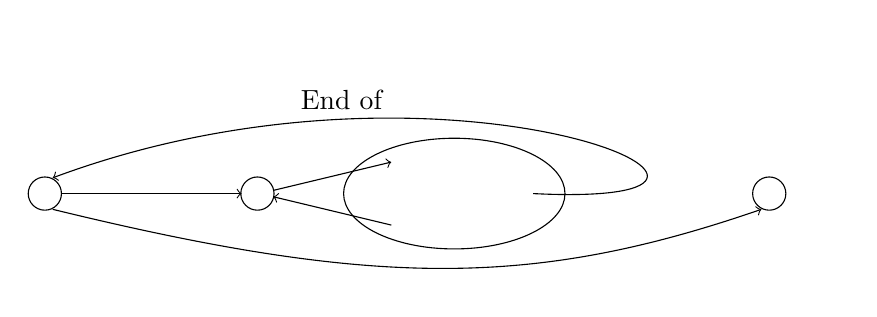
\begin{tikzpicture}
\draw (1.8,0) ellipse (6pt and 6pt) node {} ;
\draw (4.5,0) ellipse (6pt and 6pt) node {};
\draw[->] (2,0) -- (4.3,0)  node[midway,above] {~~~};
  \draw[->] (4.7,0.04) -- (6.2,0.4);
\draw[<-] (4.7,-0.04) -- (6.2,-0.4);
\draw (7,0) ellipse (40pt and 20pt) node {};
\draw (11,0) ellipse (6pt and 6pt) node {};
\draw[->] (8,0) .. controls (12,-0.2) and (7,2.1)  .. (1.9,0.2) node[near end,above] {End of };
\draw[->] (1.9,-0.2) .. controls (6,-1.2) and (8,-1.2)  .. (10.9,-0.2) node[midway,below] {};

\end{tikzpicture}
\caption{Labels of while}\label{fig:labwhile}
\end{figure}
}




\n{\figthun}{
\begin{figure}
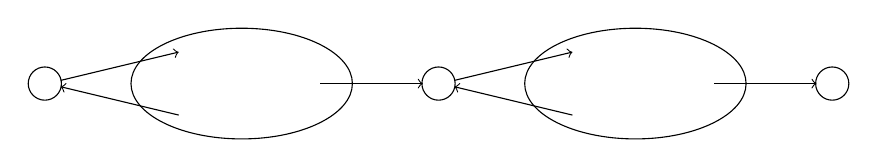
\begin{tikzpicture}
\draw (-0.5,0) ellipse (6pt and 6pt) node {} ;
\draw[->] (-0.3,0.04) -- (1.2,0.4);
\draw[<-] (-0.3,-0.04) -- (1.2,-0.4);
\draw (2,0) ellipse (40pt and 20pt) node {};
\draw (4.5,0) ellipse (6pt and 6pt) node {};
\draw[<-] (4.3,0) -- (3,0);
\draw[->] (4.7,0.04) -- (6.2,0.4);
\draw[<-] (4.7,-0.04) -- (6.2,-0.4);
\draw (7,0) ellipse (40pt and 20pt) node {};
\draw (9.5,0) ellipse (6pt and 6pt) node {};
\draw[<-] (9.3,0) -- (8,0);
\end{tikzpicture}
\caption{Labels of sequences}\label{fig:labseq}
\end{figure}
}


\n{\mytable}{\begin{floatingtable}[r]{
\begin{tabular}{l|c|c|c|c|}
& \loc & \progint & \multicolumn{2}{c|}{\progP} \\ \cline{3-5}
& & time & time & \begin{tabular}{l}false\\ alarms\end{tabular} \\
\hline
\messag & 65 & 0.05 & 0.20s & 0 \\
\hline
\embarque & 27 100 & - & 0.34s & 7 \\
\hline
\douze & 342 & - & 3.7s & 1 \\
\hline
\quinze & 414 & 3.8  & - & - \\
\hline
\end{tabular}} \caption{Benchmarks}\label{table:benchmarks}
\end{floatingtable}
}


\n{\tableabstraction}{
\begin{floatingtable}{\small \begin{tabular}[r]{|p{4.82cm}|p{2.6cm}|}
 Concrete function & Abstract function\!\!\\
 \hline
 &  \!\!\\
 \hline
 &\!\!\\
 \hline
  & \!\!\\
 \hline
  & \!\!\\
 \hline
\end{tabular}\vspace{-2mm}}\caption{Given abstractions\vspace{-2mm}}\label{fig:abstractions}
\end{floatingtable}
}


\n{\examples}{\begin{figure}{\nlnew \subfloat[]{\label{subfig:while}
}
\subfloat[]{\label{subfig:create}

}\\
\subfloat[]{\label{subfig:exemple}

} 
\subfloat[]{\label{fig:example:inter}\begin{tabular}{l}
 \\
\\

\end{tabular}}
}\caption{Program Examples}\label{fig:examples}
\end{figure}
}


\n{\myexamplebis}{
\begin{floatingfigure}{3.3cm}\hspace{-9mm}
\fbox{\hspace{-1mm}
\begin{tabular}{l}
 \\
\\

\end{tabular}\hspace{-2mm}
}
\caption{Example}\label{fig:example:inter}
\end{floatingfigure}
}

\n{\myexample}{
\begin{floatingfigure}{3.5cm}\hspace{-9mm}
\fbox{\hspace{-1mm}
\begin{tabular}{l}
 \\
\\

\end{tabular}\hspace{-2mm}
}
\caption{Example}\label{fig:example}
\end{floatingfigure}
}


\n{\subformulareach}{(\restrict{\concr{G}}{\after(\sinit)}\cap\TR{\lab \stmt,\ell'})\cup \restrict{\concr{A}}{\compl{\after(\sinit)}}
}

\n{\formulareach}[1][\send]{\left\{(\sinit,#1)\left|
\begin{array}{l}
 (\sinit,#1) \in \big[
\subformulareach
\big]^{\star}
\\
 \wedge \thread(\sinit)=\thread(#1) \wedge \lbl(\sinit)=\ell
\end{array}
\right.\right\}}

\n{\formaldefsem}{\begin{definition}\label{def:concrsem}
where:
 \send,\sinter)\in \ext{s_0}{s_1} \wedge \sinter\in\after(\sinit)\smallsetminus \after(\send)\end{array}
\right.\right\}
 \thread(i,P,\m,\h) \egdef i\lbl(i,P,\m,\h) \egdef P(i) \after(i,P,\m,\h)\egdef\{(j,P',\m',\h\cdot\h')\in\St| j\in\desce_{\h'}(\{i\}) \} X\subset \wp(\ids)\desce_{\epsilon}(X) \egdef X\desce_{(i,\ell,j)\cdot\h}(X)\egdef
 \begin{cases}
  \desce_{\h}(X\cup\{j\}) & \text{if }i\in X\\  
  \desce_{\h}(X) & \text{else}
 \end{cases}
  \begin{array}{cc}\hspace{-0.25cm}
 \regle[\hspace{-0.1cm}assign]{\m'= \ecr_{lv:=e}(\m)}{\li1 lv:=e,\ell_2 \vdash (\ell_1,\m) \rightlocarrow (\ell_2,\m') }
& 
\hspace{-0.15cm}\regle[\hspace{-0.06cm}guard]{\evb(\m,\cond)=\vrai}{\hspace{-0.1cm}\li1 \cguard(\cond),\ell_2 \vdash
(\ell_1,\m)\rightlocarrow(\ell_2,\m)}
\end{array}\begin{array}{cc}\hspace{-0.2cm}
\regle[while entry]
{\li1 \cguard(\cond),\ell_2\vdash t}
{\li1 \cwhile(\cond)\{\li2\cmd\},\ell_3\vdash t}
&
\regle[while exit]
{\li1 \cguard(\guardn),\ell_3\vdash t}
{\li1 \cwhile(\guardp)\{\li2\cmd\},\ell_3 \vdash t}
\end{array}\regle[then]
{\li1 \cguard(\guardp),\ell_2\vdash t}
{\li1 \cifte{\guardp}{\{\li2\cmd_1\}}\{\li3cmd_2\},\ell_4 \vdash t}\regle[else]
{\li1 \cguard(\guardn),\ell_3\vdash t}
{\li1 \cifte{\guardp}{\{\li2\cmd_1\}}\{\li3cmd_2\},\ell_4 \vdash t}\regle[parallel]{P(i)=\ell  \sepprem \li1 \stmt,\ell_2\vdash (\ell,\m)\rightlocarrow (\ell',\m') }{
\li1 \stmt,\ell_2\Vdash (i,P,\m,\h) \rightarrow (i,
\fx{P}{i}{\ell'}
,\m',\h)
}\regle[spawn]{ P(i)=\ell_1 \sepprem \text{ is fresh 
in }\sepprem P'=\fx{ \fx{P}{i}{\ell_{3}} }{j}{\ell_2} }{\li1\crcreate(\ell_2),\ell_3 \Vdash
(i,P,\m,\h) \rightarrow (i,
P'
,\m,h\cdot (i,\ell_2,j))}\regle[then body]{\li2\cmd,\ell_4\Vdash \tau }{\li1 \cifte{\guardp}{\{\li3\cmd_2\}}\{\li3cmd_2\},\ell_4 \Vdash \tau}
\regle[else body]{\li2\cmd,\ell_4\Vdash \tau }{\li1 \cifte{\guardp}{\{\li2\cmd_1\}}\{\li3cmd_2\},\ell_4 \Vdash \tau}
\begin{array}{ccc}
\regle[create]{\li1\crcreate(\ell_2),\ell_{3} \Vdash\tau}{\li1\ccreate(\li2\cmd),\ell_{3} \Vdash\tau}&\quad&
\regle[while body]{\li2\cmd,\ell_1\Vdash \tau }{\li1 \cwhile(\cond)\{\li2\cmd\},\ell_3 \Vdash \tau}
\end{array}\begin{array}{ccc}
\regle[sequence 1]{\li{1}\cmd_1,\ell_{2}\Vdash \tau }{\li1 \cmd_1;\li2\cmd_2,\ell_3 \Vdash \tau}
&\quad&
\regle[sequence 2]{\li{2}\cmd_2,\ell_{3}\Vdash \tau }{\li1 \cmd_1;\li2\cmd_2,\ell_3 \Vdash \tau}
\end{array}\begin{array}{ccc}
\regle[child]{\li2\cmd,\lend\Vdash \tau }{\li1 \ccreate(\li2\cmd),\ell_3 \Vdash \tau}
&\quad&
\regle[schedule]{
\text{ is defined}\sepprem i\neq j}
{
\lab \stmt,\ell'\Vdash (i,P,\m,\h)\rightarrow(j,P,\m,\h)
}\end{array} 
 \hspace{-0.5cm}\begin{array}{cclr}
 lv & ::= \pluspres&\pluspres & \text{left value}\\
  & |\pluspres &\pluspres x & \text{variable}\\
  & |\pluspres &\pluspres\pluspres {}^{\ast}e\hspace{-1cm} & \hspace{-1cm}\text{pointer deref}\\
e & ::= \pluspres&\pluspres & \hspace{-1cm}\text{expression}\\
 & |\pluspres & c & \text{constant}\\
 & |\pluspres &\pluspres lv & \text{left value}\\
 & |\pluspres &\pluspres o(e_1,e_2)\hspace{-0.3cm} & \text{operator}\\
 & |\pluspres &\pluspres \&x &\text{address}\\
\cond & ::= & &\pluspres \hspace{-1cm}\text{condition}\\
 & |\pluspres &\pluspres x & \text{variable}\\
 & |\pluspres &\pluspres \neg \cond\hspace{-0.3cm} & \text{negation}\\
 \end{array}
 \begin{array}{cclr}
 \cmd & ::= \pluspres& \pluspres&\pluspres \text{command}\\
 & |\pluspres &\pluspres \lab lv := e & \text{assignment}\\
 & |\pluspres &\pluspres \cmd_1;\cmd_2\hspace{-1cm} & \text{sequence}\\
 & |\pluspres &\pluspres \cifte{\cond}{\{\cmd_1\}}\{\cmd_2\} \hspace{-1.8cm}& \text{if}\\
 & |\pluspres &\pluspres \lab \cwhile(\cond)\{\cmd\}\hspace{-1cm}&\text{while}\\
 & |\pluspres &\pluspres \lab \ccreate(\cmd)&\text{new thread}\\
\stmt & ::= \pluspres& \pluspres& \text{statement}\\
 & |\pluspres &\pluspres \cmd,\ell' & \text{command}\\
 & |\pluspres &\pluspres \lab \cguard(\cond),\ell' & \text{guard}\\
 & |\pluspres &\pluspres \lab \crcreate(\ell''),\ell'&\text{new thread}\\
\end{array}
\begin{array}{rcl}
\asem{\lab lv:=e} \milieu  \assign{lv:=e}\abstr{Q} \\ 
\asem{\li{1}\cmd_1;\li{2}\cmd_2} \milieu \asem{ \li{2}\cmd_2}\circ \asem{\li{1}\cmd_1} \abstr{Q} \\
\asem{\li1\cwhile(\guardp)\{\li2\cmd\}} \milieu \guard{\guardn} \loopwa\eomega \abstr{Q}\\
\text{with } \loopwa (\abstr{Q'}) &\egdef& \big(\asem{\cmd} \circ \guard{\guardp} \abstr{Q'}\big)\sqcup\abstr{Q'}\\
\asem{\li1\ccreate(\li2\cmd)}\milieu \glue{\abstr{Q}'}\circ \afp{\li2\cmd}\eomega \circ \afinit{\ell_2} (\abstr{Q})
\\
\text{with } \abstr{Q'} &\egdef& \aspawn{\ell_2}(\abstr{Q})
\end{array}\asem{\li0\cpar\{\li1\cmd_1|\li2\cmd_2\}}(\abstr{Q})\egdef\langle \abstr{C_1}\sqcap\abstr{C_2},\abstr{L},
\abstr{K'}
,\abstr{I}_1\sqcup\abstr{I}_2  \rangle\qup{_1}= \afp{\li1\cmd_1,\lend} \circ \afinit{\ell_1} (\abstr{Q})  \qup{_2}= \afp{\li2\cmd_2,\lend} \circ \afinit{\ell_2} (\abstr{Q})  \abstr{K'}=\fx{\fx{\abstr{K}}{\ell_1}{\abstr{K_2}(\fin)\sqcup\abstr{K}(\ell_1)}}{\ell_2}{\abstr{K}_1(\fin)\sqcup\abstr{K}(\ell_2)}\hspace{-0.2cm}\begin{array}{rcl}
  \cinter{\concr{A}}(\concr{S})&\egdef& \left\{s'\left| \exists s\in\concr{S}  :
   \begin{array}{l} 
   (s,s')\in(  \restrict{\concr{A}}{\compl{\after(s)}}\cup\Sche)^{\star}
   \\
   \wedge \thread(s)=\thread(s')
   \end{array}
     \right. \right\}
  \\
  \cextract{\ell}&\egdef&\left\{s'\left| \begin{array}{l}\exists s = (i,P,\m,\h\cdot(i,\ell,j))\in\St : \\  s'\in\after(s)\end{array}\right.\right\}
  \\
   \cschedule(\concr{S}) &\egdef& \left\{(j,P,\m,\h')\left| \exists i,\h : \begin{array}{l}(i,P,\m,\h')\in \concr{S}\\ \wedge \h'=\h\cdot(i,\ell,j)\end{array}\right.\right\}
   \\
\cinit_{\ell}(\qc)&\egdef  &
 \langle \cinter{\concr{A}\cup (\restrict{\concr{G}}{\cextract{\ell}})}\circ \cschedule(\concr{S}),\\ & & {}\quad\Sche,
  \concr{A}\cup(\restrict{\concr{G}}{\cextract{\ell}}) \rangle
 \\
 \ccomb_{\qc}(\concr{G}')&\egdef&  \langle \cinter{\concr{A}\cup\concr{G}' }(\concr{S}),\concr{G}\cup\concr{G}'
, \concr{A}\cup\concr{G}'  \rangle
\\
\cexe_{f,\concr{S},\concr{A}}(\concr{\concr{G}}) &\egdef& \concr{G}' \text{ with } \langle \concr{S}',\concr{G'},\concr{A}'\rangle = f \qc
\\
\fpd{f}\qc &\egdef& \cexe_{f,\concr{S},\concr{A}}\eomega (\concr{G})
   \end{array} \fx{f}{z}{t} f z  t  \nf{f}{z}{t} f z t\ndf{f}{x}f(x) \fx{f}{z}{t} f z  t \cpar\ccreate\cpar\cmd\stmt\cmd,\ell'\ell_3\nr[a2]\ccreate(\nr[a3] x:=x+1),\nlrefb{a1}\Lab\lab \stmt,\ell'\ell\ell'\ell_2x:=x+1\ell_3\lend\cmd_1;\cmd_2\nlref{init2}\lab \cmd\cmd\ell\lab \stmt,\ell'\stmt\ell\ell'\lab \cmd,\lend\ccreate\cwhile\cif\cwhile\li1\crcreate(\ell_2),\ell_3\li1\cguard(\cond),\ell_2\ccreate\cwhile\cif\li1\crcreate(\ell_2),\ell_3\li1\cguard(\cond),\ell_2\ids\main \in\idsP\mainP\mathbb{P}\dom(P)P\fx{P}{i}{\ell}\fx{P}{i}{\ell}(j)\egdef
\begin{cases}
 \ell & \text{if }i=j\\
 P(j) &\text{if }i\in\dom(P)\smallsetminus\{j\}\\
 \text{undefined}& \text{else}\\
\end{cases}
i,\ell,j)\in\ids\times\Lab\times\idsi_1,\ell_1,j_1)i_2,\ell_2,j_2)j_1\neq j_2\maini,\ell,j)ij\ellj\hi,\ell,j)\h\Hist\h\cdot \h'\h\h'\main\stores\ecr_{lv:=e}(\m)\evb(\m,\cond)\m\ecr_{lv:=e}lv:=e\evb\cond\m\vrai\faux\cstate{}\in\ids\times \mathbb{P}\times \stores \times \Histi\in\dom(P)\dom(P)\{\main\}\h\St (i,P,\m,\h)iP\m\h\dom(P)P\h\li0\cmd,\lend\ini (\main,P_0 , \m,\epsilon)\dom(P_0)=\{\main\}P_0(\main)=\ell_0\m\epsilon\tau=\big((i,P,\m,\h),(i',P',\m',\h\cdot\h')\big)\forall j\in\dom(P)\smallsetminus\{i\}, P(j)=P'(j)j,\ell,j')\h'j=iP(i)=\ell\Tra\Sche\egdef\{((i,P,\m,\h),(j,P,\m,\h))\in\Tr\mid i\neq j \}\Sches_1\rightarrow s_2 s_1s_2 \li1 \stmt,\ell_2 \Vdash s_1 \rightarrow s_2s_1\rightarrow s_2 \cmd\ell'\li1 \stmt,\ell_2 \vdash (\ell,\m)\rightarrow(\ell',\m')\li1\cwhile(x)\{\li2\ccreate(\li3x:=0)\}ji,P,\m,\h)i\neq jP(j)j\h\hi,\ell,i')ii'j\h\lab{}\stmt,\ell'\TR{\lab{}\stmt,\ell'}=\{(s,s')\mid\lab \stmt,\ell'\Vdash s\rightarrow s' \}.\nlref{init1}\excmd_1,\lend\ids\mathbb{P}\TR{\lab{}\stmt,\ell'}\stores\TR{\lab{}\stmt,\ell'}[x=n]xn
 \TR{\nr[init1] x:=0,\nlref{a1}}=&\{((i,P,[x=n],\h),(i,\fx{P}{i}{\nlrefb{a1}},[x=0],\h))\mid P(i)=\nlrefb{init1}\\& \wedge i\in\ids\wedge n\in\mathbb{Z}\}.\\
 \TR{\nr[a3] x:=x+1,\lend}=&
  \{((i,P,[x=n],\h),(i,\fx{P}{i}{\lend},[x=n+1],\h))\mid P(i)=\nlrefb{a3} \\&\wedge i\in\ids\wedge n\in\mathbb{Z}\}.
\Labs{\lab \cmd,\lend}\lab \cmd,\lend\Labss{\cdot}\Labss{\li1\ccreate(\li2\cmd),\ell_3}=\Labs{\li2\cmd,\lend}\Labss{\li1\cmd_1,\li2\cmd_2,\ell_3} = 
 \Labss{\li1\cmd_1,\ell_2}
\cup 
 \Labss{\li2\cmd_2,\ell_3}
 \Labss{\li1\cifte{\guardp}{\{\li2\cmd_1\}}{\{\li3\cmd_2\}},\ell_4}=\\{}\quad\Labss{\li2\cmd_1,\ell_4}\cup\Labss{\li3\cmd_2,\ell_4}\Labss{\li1\cwhile(\guardp)\{\li2\cmd\},\ell_3}=\Labss{\li2\cmd_1,\ell_1}\Labss{\li1basic,\ell_2}=\emptysets,s')\in\TR{\lab\stmt,\ell'}\smallsetminus \Sche\lbl(s)\in\Labs{\lab\stmt,\ell'}\smallsetminus\{\ell'\}\lbl(s')\in\Labs{\lab\stmt,\ell'}\thread(s)=\thread(s')\lbl(s)\notin \Labs{\lab \stmt ,\ell'}\smallsetminus\{\ell'\}s's,s')\notin\TR{\lab\stmt,\ell'}\smallsetminus \Sche\lab\stmt,\ell'\Labss{\lab\stmt,\ell'}s,s')=(\cstate{},\cstate{'})\in\TR{\lab\stmt,\ell'}\smallsetminus \Schej\in\dom(P')\smallsetminus\dom(P)P'(j)\in \Labss{\lab\stmt,\ell'}\subset\Labs{\lab\stmt,\ell'}s,s')\in\TR{\lab\stmt,\ell'}\smallsetminus \Sche\lbl(s)\in\Labss{\lab\stmt,\ell'}\smallsetminus\{\ell'\}\lbl(s')\in\Labs{\lab\stmt,\ell'}\ell\notin\Labs{\lab\stmt,\ell'}\ell'\notin\Labs{\lab\stmt,\ell'}\li1 lv:=e,\ell_2\li1\cguard(\cond),\ell_2\li1 \cspawn(\ell_3),\ell_2 \li1 basic,\ell_2s,s')=(\cstate{},\cstate{'})\in \TR{\li1 basic,\ell_2}\smallsetminus\Sche\thread(s)=\thread(s')\lbl(s)=\ell_1\lbl(s')=\ell_2\concr{Q}=\qc\concr{S}\concr{G}\concr{A}\concr{S}\concr{G}\concr{A}\Sche\qcp{_1}\leqslant\qcp{_2} \Leftrightarrow \concr{S_1}\subset\concr{S_2}\wedge\concr{G_1}\subset\concr{G_2}\wedge\concr{A_1}\subset\concr{A_2}  \main=j_0\sinit\thread(\sinit)\sinitj_0\sinterj_2j_0j_1j_1j_0j_0j_1j_1j_3j_3j_0j_1j_0\sinit=(j_0,\Pinit,\minit,\hinit)\hinit=[(j_0,\ell_1,j_1)]j_0\hinit\desce_{\hinit}(\{j_0\})\{j_0,j_1\}\sinter\hinit\cdot \hinterf\hinterf\hinterf=[(j_0,\ell_2,j_2),(j_1,\ell_3,j_3),(j_2,\ell_4,j_4)]\sinterj_0\hinit\cdot \hinterf\desce_{\hinit\cdot\hinterf}(\{j_0\})=\{j_0,j_1,j_2,j_3,j_4\}\hinterfj_2j_3\h\cdot\h'ij\h'\desce_{\h'}(\{j\}) \subset \desce_{\h\cdot\h'}(\{i\}) \desce_{\h'}(\{j\}) \cap \desce_{\h\cdot\h'}(\{i\}) = \emptyset\h'\h'=\epsilon\desce_{\epsilon}(\{j\}) = \{j\} \h'=\h''\cdot(i',\ell,j')\desce_{\h''}(\{j\}) \subset \desce_{\h\cdot\h''}(\{i\}) \desce_{\h''}(\{j\}) \cap \desce_{\h\cdot\h''}(\{i\}) = \emptyseti'\in \desce_{\h''}(\{j\})j'\in \desce_{\h''\cdot(i',\ell',j')}(\{j\})j'\in \desce_{\h\cdot\h''\cdot(i',\ell',j')}(\{i\})j'\notin \desce_{\h''\cdot(i',\ell',j')}(\{j\})i'\in \desce_{\h''}(\{j\})i'\notin \desce_{\h\cdot\h''}(\{i\})j\h\cdot\h''j\notin \desce_{\h\cdot\h''}(\{i\})j'\in \desce_{\h''\cdot(i',\ell',j')}(\{j\})j'\notin \desce_{\h\cdot\h''\cdot(i',\ell',j')}(\{i\})i'\in \desce_{\h\cdot\h''}(\{i\})i'\notin\desce_{\h''}(\{j\})\cup \desce_{\h\cdot\h''}(\{i\})\desce_{\h\cdot\h''\cdot(i',\ell',j')}(\{i\}) = \desce_{\h\cdot\h''}(\{i\})  \desce_{\h''\cdot(i',\ell',j')}(\{j\}) = \desce_{\h''}(\{j\})\hinterfj_1j_0\desce_{\hinterf}(\{j_0\})=\{j_0,j_2,j_4\}j_3\notin \desce_{\hinterf}(\{j_0\})j_3\hinterf\sinit=(j_0,\Pinit,\minit,\hinit)j_0\sinitj_0j_0j_0\after(\sinit)\after(\sinit)\afterTs_0,s_1)\in T^{\star}\thread(s_0)=\thread(s_1)s_1\in\after(s_0)s_1\in\after(s_0)\after(s_1)\subset\after(s_0)\cstate{_0}=s_0\cstate{_1}=s_1\h'_1\h_1=\h_0\cdot\h'_1i_0\in\desce_{\epsilon}(\{i_0\})i_0\in\desce_{\h'_1}(\{i_0\})\thread(s)=\thread(s')i_1=i_0s_1\in\after(s_0)\afters_1\in\after(s_0)s_2=\cstate{_2}\in\after(s_1)\h'_2\h_2=\h_1\cdot\h'_2=\h_0\cdot\h'_1\cdot\h'_2i_2\in\desce_{\h'_2}(\{i_1\})s_1\in\after(s_0)i_1\in\desce_{\h'_1}(\{i_0\})i_1\in\desce_{\h'_2}(\{i_1\})\cap\desce_{\h'_1\cdot\h'_2}(\{i_0\})\desce_{\h'_2}(\{i_1\})\subset\desce_{\h'_1\cdot\h'_2}(\{i_0\})i_2\in\desce_{\h'_1\cdot\h'_2}(\{i_0\})s_2\in\after(s_0)s_1,s_2)\in \Sche\after(s_1)\cap\after(s_2)=\emptyset\cstate{_1}=s_1i_2=\thread(s_2)i_2,P_1,\m_1,\h_1)=s_2s=\cstate{}\in \after(s_1)\cap\after(s_2)\after\h'\h=\h_1\cdot\h'i\in \desce_{\h'}(\{i_1\})i\in \desce_{\h'}(\{i_2\})i_1i_2\dom(P_1)i_1i_2\h_1\maini_1i_2\h'i_2\notin\desce_{\h'}(\{i_1\})\desce_{\h'}(\{i_2\})\subset\desce_{\epsilon\cdot\h'}(\{i_1\})\desce_{\h'}(\{i_1\})\cap\desce_{\h'}(\{i_2\}) = \emptyseti\in \desce_{\h'}(\{i_1\})i\in \desce_{\h'}(\{i_2\})TTs,s')=(\cstate{},\cstate')\in T, \h=\h's_0=\cstate{_0}s=(i,P,\m,\h_0\cdot\h)s=(i',P',\m',\h_0\cdot\h\cdot\h')s,s')\in( \restrict{\concr{A}}{\compl{\after(s_0)}}\cup T)^{\star}\desce_{\h\cdot\h'}\{i_0\}=\desce_{\h}\{i_0\}s_1,\ldots,s_ns_1=sk\in\{1,\ldots,n-1\}s_k,s_{k+1)}\in \restrict{\concr{A}}{\compl{\after(s_0)}}\cup T)^{\star}s_n=s'i_k,P_k,\m_k,\h_0\cdot\h\cdot\h_k)=s_k\h_k\neq\h_{k+1}s_k,s_{k_1})\in\restrict{\concr{A}}{\compl{\after(s_0)}}i_k\notin \desce_{\h\cdot\h_k}\{i_0\} \desce_{\h\cdot\h_k}\{i\}=\desce_{\h\cdot\h_{k+1}}\{i_0\}\desce_{\h\cdot\h_k}\{i\}=\desce_{\h\cdot\h_{k+1}}\{i\}\desce_{\h\cdot\h'}\{i\}=\desce_{\h}\{i\}Ts,s')=(\cstate{},\cstate')\in T, \h=\h's=(i,P,\m,\h)s=(i',P',\m',\h\cdot\h')s,s')\in( \restrict{\concr{A}}{\compl{\after(s_0)}}\cup T)^{\star}\desce_{\h'}\{i\}=\{i\}s_0=s\afterTs,s')=(\cstate{},\cstate')\in T, \h=\h's_0,s_1)\in( \restrict{\concr{A}}{\compl{\after(s_0)}}\cup T)^{\star}s_1\in\after(s_0)\thread(s_1) = \thread(s_0)\cstate{_0} =s_0 i_1,P_1,\m,\h_0\cdot\h_1)=s_1\desce_{\h_1}\{i_0\}=\{i_0\}\afteri_1\in \desce_{\h_1}\{i_0\}T_1s,s')=(\cstate{},\cstate')\in T, \h=\h'T_2s_0,s_1,ss_0,s_1)\in T_1^{\star}\thread(s_0)=\thread(s_1)s_1,s)\in T^{\star}s\in\after(s_0)s\in\after(s_1)\cstate{_0} =s_0 i_1,P_1,\m,\h_0\cdot\h_1)=s_1i,P,\m,\h_0\cdot\h_1\cdot\h)=s\desce_{\h_1}\{i_0\}=\{i_0\}\afteri_1\in \desce_{\h_1}\{i_0\}\desce_{\h_1\cdot\h}(\{i_0\}) = \desce_{\h}(\desce_{\h_1}(\{i_0\})) = \desce_{\h}(\{i_0\})s\in\after(s_0)i\desce_{\h_1\cdot\h}(\{i_0\})i\desce_{\h}(\{i_0\})s\in\after(s_1)R\restrict{R}{S}=\{(s,s')\in R \mid s\in S\}RSR\langle S \rangle=\{s'\mid\exists s\in S : (s,s')\in R\}RSR ; R' =\{(s,s'') \mid\exists s'\in\St : (s,s')\in R \wedge (s',s'')\in R' \}RR'R^{\star} = \bigcup_{k\in\mathbb{N}}R^{k}R^{0}=\{(s,s) \mid s\in\St\}R^{k+1}=R; R^{k}S\compl{S}=\St\smallsetminus S\concr{S}\osem{\lab \stmt,\ell'}\lab \stmt,\ell'\sinit=(j_0,P,\m,\h)\send=(j_0,P',\m',\h\cdot \h')\lab \stmt,\ell'j_5\nr[b1] y:=0;\nlref{b2}\sinter\sinit\sinit\sinter\concr{G}\concr{S'}\concr{S}
 \col&=\{(\sinit,\send)\in\big[\concr{G}\cap \TRi{\lab \stmt,\ell'} \big]^{\star}| \lbl(\sinit)=\ell\}\\
 \concr{S}' &= \{\send \mid \send\in\col(\concr{S}) \wedge \lbl(\send)=\ell' \} \\
 \Se&=\{(\sinter,\sinterb)\in \TRi{\lab \stmt,\ell'} \mid \sinter\in \col(\concr{S}) \}\\
 \av{\lab \stmt,\ell'}&\langle \concr{S}, \concr{G} , \Sche \rangle = \langle \concr{S}',
 \concr{G}\cup\Se,
 \Sche   \rangle \vspace{-1.5mm}
 \Su&=\Sud=\emptyset
 j_0j_1j_3\concr{A}\li{_{\ref{label:un}}} y:= 1; \li{_{\ref{label:deux}}} z:=y,\lendz3\li{_{\ref{label:trois}}}y:=3,\lend\main\ell_{\ref{label:deux}}\concr{A}\col\lab \stmt,\ell'j_0\after(\sinit)j_1j_3\compl{\after(\sinit)}\col = \formulareach. j_0\lab \stmt,\ell'j_2j_4\concr{G}\Su\Sche\circ\col(\{s_0\})\after(\sinit)\Su = 
\{(\sinter,\sinterb)\in\TRi{\lab \stmt,\ell'}\mid \exists \sinit\in\concr{S} : ( \sinit,\sinter)\in \Sche\circ \col \wedge \sinter\in\after(\sinit) \}.
j_0\lab \stmt,\ell'\sendiij_4j_5j_6\Su\Sudi\ccreate\sinit\sends,s')\after(\sinit)\smallsetminus\after(\send)\sends\restrict{\concr{G}}{\after(\sinit)}\cap\TRi{\lab \stmt,\ell'})\cup \restrict{\concr{A}}{\compl{\after(\sinit)}}\colj_0j_5\restrict{\concr{G}}{\after(\send)}fDX\subset DX \subset f(X)ff\eomega(X)\egdef\bigcup_{n\in\mathbb{N}}f^n(X)\cinter{\concr{A}}(\concr{S})\concr{S}\concr{A}s=\cstate{}s'=\cstate's,s') \in ( \restrict{\concr{A}}{\compl{\after(s)}}\cup\Sche )^{\star}P(i)=P'(i)\lbl(s)=P'(\thread(s))\thread(s)=\thread(s')\lbl(s)=\lbl(s')s_0s_ns_0=ss_n=s'k\in\{0,\ldots,n-1\}s_k,s_{k+1})\in \restrict{\concr{A}}{\compl{\after(s)}}\cup\Sche\cstate{_k}=s_kP_k(i)=P(i)s_k,s_{k+1})\in\ScheP_k(i)=P(i)P_{k+1}(i)=P(i)s_k,s_{k+1})\in \restrict{\concr{A}}{\compl{\after(s)}}P_k(i)=P(i)s_k\notin\after(s_k)i_k\neq iP_{k+1}(i)=P_{k}(i)=P(i)\cextract{\ell}\ell\cschedule\cinit_{\ell}\ell\cextract{\ell}\cextract{\ell}\cexef\fp{}\cexe\lab\stmt,\ell's_0,s)\in (\TR{\lab\stmt,\ell'}\cup\restrict{\concr{A}}{\compl{\after(s_0)}})^{\ast}\lbl(s_0)\in\Labs{\lab\stmt,\ell'}s\in\after(s_0)\lbl(s)\in \Labs{\lab\stmt,\ell'}\lbl(s)=\ell'\lbl(s)=\ell\thread(s_0)=\thread(s)s_1,\ldots,s_ns_n=sk\in\{0,\ldots,n-1\}s_k,s_{k-1})\in \TR{\lab\stmt,\ell'}\cup\restrict{\concr{A}}{\compl{\after(s_0)}}\cstate{_0}=s_0k\geqslant 1i_k,P_k,\m_k,\h_0\cdot\h_k)=s_kkP_{k}(i)\in\Labs{\lab\stmt,\ell'}j\in\desce_{\h_k}(\{i_0\})\smallsetminus\{i_0\}P_{k}(j)\in\Labss{\lab\stmt,\ell'}kk+1s_k,s_{k+1})\in\restrict{\concr{A}}{\compl{\after(s_0)}}i_k\notin\desce_{\h_k}(\{i_0\})j=\desce_{\h_k}(\{i_0\})=\desce_{\h_{k+1}}(\{i_0\})P_k(j)=P_{k+1}(j)s_k,s_{k+1})\in\TR{\lab\stmt,\ell'}i_k=i_0P_{k+1}(i_k)\in\Labs{\lab\stmt,\ell'}j\in\desce_{\h_k}(\{i_0\}) P_k(j)=P_{k+1}(j)j\in\desce_{\h_{k+1}}(\{i_0\})\smallsetminus\desce_{\h_k}(\{i_0\})j\in\dom(P_{k+1})\smallsetminus\dom(P_k)P_{k+1}(j)\in \Labss{\lab\stmt,\ell'}s_k,s_{k+1})\in\TR{\lab\stmt,\ell'}i_k=i_0s\in\after(s_0)i_n\in\desce_{\h_n}(\{i_0\})\lbl(s)\in \Labs{\lab\stmt,\ell'}\lbl(s)=\ell'\lbl(s)=\ell\ell\ell'\Labss{\lab \stmt,\ell'}\thread(s_0)=\thread(s)\col\nq = \ssem{\lab\stmt,\ell'}\qcs_0,s)\in\cols\in\after(s_0)\after(s)\subset\after(s_0)\lbl(s)\in\Labs{\lab\stmt,\ell'}s_0,s)\in\big[\subformulareach\big]^{\star} s\in\after(s_0)\after(s)\subset\after(s_0)\lbl(s)\in\Labs{\lab\stmt,\ell'}\fpd{}\fpd{}\qc\lab \stmt,\ell'\concr{G}_{\infty} = \fp{\av{\lab \stmt,\ell'}}\qcs_0\in\concr{S}s\in\after(s_0)s,s')\in \TRi{\lab \stmt,\ell'}s_0,s)\in  \big[
\restrict{(\TRi{\lab \stmt,\ell'})}{\after(s_0)}\cup \restrict{\concr{A}}{\compl{\after(s_0)}}
\big]^{\star}s,s') \in \concr{G}_{\infty}\qcp{_k} = \cexe_{\osem{\lab \stmt ,\ell'},\concr{S},\concr{A}}^k \concr{G}\nqp{_{k}} = \osem{\lab \stmt ,\ell'} \langle \concr{S} , \concr{G}_k , \concr{A}  \rangle T= \TRi{\lab \stmt,\ell'}s_0,\ldots,s_{n+1}s_n=ss_{n+1}=s'ks_k,s_{k+1}) \in \big[\restrict{T}{\after(s_0)}\cup \restrict{\concr{A}}{\compl{\after(s_0)}}
\big]^{\star}mk_0ks_{k},s_{k+1}) \in \restrict{T}{\after(s_0)}\smallsetminus \concr{G}_{m} s_{k},s_{k+1})\in \Se_{m}\cup\Su_{m}\subset \concr{G}_{m+1}\subset\concr{G}_{\infty}\li1 basic,\ell_2\nq=\ssem{\li1 basic,\ell_2} \qc s_0,s) \in \cols \in \cinter{\concr{A}}(\{s_0\})\lbl(s)=\ell_1s \in\cinter{\concr{A}}(\TR{\li1 basic,\ell_2} \smallsetminus\Sche \langle \cinter{\concr{A}}(\{s_0\}) \rangle)\lbl(s)=\ell_2s_0,s) \in (\restrict{\concr{A}}{\compl{\after(s_0)}}\cup\Sche)^{\star}\col\thread(s_0)=\thread(s)s \in \cinter{\concr{A}}(\{s_0\})\lbl(s_0)=\lbl(s)\lbl(s)=\ell_1s_0,s) \notin (\restrict{\concr{A}}{\compl{\after(s_0)}}\cup\Sche)^{\star}s_0,s)\in\cols_0,s) \in [(\restrict{\concr{G}}{{\after(s_0)}}\cap\TR{\li1 basic,\ell_2})\restrict{\concr{A}}{\compl{\after(s_0)}}]^{\star}s_0,s) \in (\restrict{\concr{A}}{\compl{\after(s_0)}}\cup\Sche)^{\star};[\restrict{\concr{G}}{{\after(s_0)}}\cap\TR{\li1 basic,\ell_2}\smallsetminus\Sche];[(\restrict{\concr{G}}{{\after(s_0)}}\cap\TR{\li1 basic,\ell_2})\restrict{\concr{A}}{\compl{\after(s_0)}}]^{\star}s_1, s_2, s_3,\ldots,s_ns_1,s_2)\in(\restrict{\concr{A}}{\compl{\after(s_0)}}\cup\Sche)^{\star} s_2,s_3)\in \restrict{\concr{G}}{{\after(s_0)}}\cap\TR{\li1 basic,\ell_2}\smallsetminus\Schek\in\{3,\ldots,n\}s_k,s_{k+1})\in (\restrict{\concr{G}}{{\after(s_0)}}\cap\TR{\li1 basic,\ell_2})\restrict{\concr{A}}{\compl{\after(s_0)}}s_1,s_2)\in \restrict{\concr{G}}{{\after(s_0)}}s_1\in\after(s_0)\thread(s_0)=\thread(s_1)s_1 \in \cinter{\concr{A}}(\{s_0\})\lbl(s_2)=\ell_2k_0k\geqslant 2s_{k},s_{k+1})\in \TR{\li1 basic,\ell_2} \smallsetminus\Sches_2,s_{k_0})\in (\restrict{\concr{A}}{\compl{\after(s_0)}}\cup\Sche)^{\star}\lbl(s_{k_0})=\lbl(s_2)=\ell_2k\in\{3,\ldots,n\}s_k,s_{k+1})\in \Sche\cup\restrict{\concr{A}}{\compl{\after(s_0)}}\thread(s_1)=\thread(s_2)\thread(s_2)=\thread(s)s_2\in\cinter{\concr{A}}(\{s_2\})\cspawn\concr{S'}\li1 basic,\ell_2\nq=\ssem{\li1 basic,\ell_2}\qc\Su=\emptysets,s')\in\Sus,s')\in\col;\Sche\langle \concr{S} \rangles_0\in\concr{S_0}s_1s_0,s_1)\in\cols_1,s)\in\Sches\in\after(s_0)\thread(s)=\thread(s')s,s_1)\in\col\thread(s)=\thread(s_1)s_1,s)\in\Sche\thread(s)\neq\thread(s_1)\Su=\emptyset\li1 basic,\ell_2\nq=\ssem{\li1 basic,\ell_2}\qc\Sud=\emptysets,s')\in\Suds_0\in\concr{S}s_1s_0,s_1)\in\cols_2,s)\in\ext{s_0}{s_1}s\in\after(s_0)\smallsetminus\after(s_1)\cstate{_0}=s_0i_1,P_1,\m_1,\h_0\cdot\h_1)=s_1s_0,s_1)\in\col\thread(s_0)=\thread(s_1)j\in\desce_{\h_1}(\{i_0\})s'_1=(j,P_1,\m_1,\h_0\cdot\h_1)s'_1\in \after(s_0)s_0,s'_1)\in (\TR{\li1 basic,\ell_2}\cup\restrict{\concr{A}}{\compl{\after(s_0)}})^{\star};(\Sche^{\star})j=\thread(s'_1)=\thread(s_0)=i_0\desce_{\h_1}(\{i_0\})=\{i_0\}i,P,\m,\h_0\cdot\h_1\cdot\h)=s\desce\h\desce_{\h_1\cdot\h}(\{i_0\})=\desce_{\h}(\{i_0\})s\in\after(s_0)i\in \desce_{\h_1\cdot\h}(\{i_0\})i=i_0s\in\after(s_1)s\in\after(s_0)\smallsetminus\after(s_1)\Sud=\emptyset\li1 basic,\ell_2\nq=\ssem{\li1 basic,\ell_2}\qc\Su\subset \{(s,s')\in\TR{\li1 basic,\ell_2}\mid s\in \cinter{\concr{A}}(\concr{S}) \}\cup\Sches,s')\in \Se\smallsetminus\Sches,s')\in \TR{\li1 basic,\ell_2} s\in\col\langle\concr{S} \rangle \sinit\in\concr{S}s_0,s)\in\cols_0,s)\in \TR{\li1 basic,\ell_2}\smallsetminus\Sche \lbl(s)=\ell_1\neq\ell_2s \in \cinter{\concr{A}}(\{s_0\}) \subset \cinter{\concr{A}}(\concr{S})\thread(s_0)=\thread(s)s,s')\in \Se\li1 basic,\ell_2\qcp'=\osem{\li1 basic,\ell_2}\qc\nq=\ssem{\li1 basic,\ell_2}\qc\concr{S}'\subset\cinter{\concr{A}} \big(\TR{\li1 basic,\ell_2}\smallsetminus \Sche \langle  \cinter{\concr{A}}(\concr{S})\rangle\big)s\in\concr{S}'\lbl(s)=\ell_2s_0\in\concr{S}s_0,s)\in\col\lbl(s)=\ell_2\neq\ell_1s \in\cinter{\concr{A}}(\TR{\li1 basic,\ell_2} \smallsetminus\Sche \langle \cinter{\concr{A}}(\{s_0\}) \rangle) \subset\cinter{\concr{A}}(\TR{\li1 basic,\ell_2} \smallsetminus\Sche \langle \cinter{\concr{A}}(\concr{S}) \rangle) \li1 basic,\ell_2\osem{\li1 basic,\ell_2}\qc \leqslant \langle \concr{S''}, \concr{G}\cup\Gnew ,\concr{A} \rangle\concr{S}'' = \cinter{\concr{A}} \big(\TR{\li1 basic,\ell_2}\smallsetminus \Sche \langle  \cinter{\concr{A}}(\concr{S})\rangle\big)\Gnew = \{(s,s')\in\TR{\li1 basic,\ell_2}\mid s\in \cinter{\concr{A}}(\concr{S})  \} \av{\li1\cmd_1;\li2\cmd_2,\ell_3}(\concr{Q}) \leqslant \av{\li2\cmd_2,\ell_3}\circ\av{\li1\cmd_1,\ell_2}(\concr{Q})\av{\li1\cifte{(\cond}{\{\li2\cmd_1\}}\{\li4\cmd_2\},\ell_3}(\concr{Q}) 
\leqslant \\
\av{\li2\cmd_1,\ell_3}\circ\av{\li1\cguard(\cond),\ell_2}(\concr{Q}) 
\sqcup
\av{\li4\cmd_2,\ell_3}\circ\av{\li1\cguard(\neg\cond),\ell_4}(\concr{Q}) \av{\li1 \cwhile(\guardp)\{\li2\cmd\},\ell_3 }(\concr{Q})\leqslant \av{\li1 \cguard(\guardn),\ell_3} \circ \loopw\eomega (\concr{Q})\loopw(\concr{Q}') = \big( \av{\li2\cmd,\ell_1} \circ 
\av{\li1  \cguard(\guardp),\ell_2} (\concr{Q}') \big) \sqcup \concr{Q'}\av{\li1\ccreate(\li2\cmd),\ell_3}(\concr{Q}) \leqslant  
\ccomb_{\concr{Q}'}\circ\fp{\av{\li2\cmd,\lend}}\circ \cinit_{\ell_2} (\concr{Q}')\concr{Q}' = \av{\li1\crcreate(\ell_2),\ell_3}(\concr{Q})\li1\ccreate(\li2\cmd),\ell_3\fp{}\lab\stmt,\ell'TT\lab\stmt,\ell's_0s_1s_2,\ldots,s_n\lab\stmt,\ell's_1\lab\stmt,\ell's_0s_1\lab\stmt,\ell'\lab\stmt,\ell'\nq=\ssem{\lab\stmt,\ell'}\qcs_0,s_1)\in\colTs,s')\in T\lbl(s)\in\Labs{\lab\stmt,\ell'}s,s')\in \TR{\lab\stmt,\ell'}s\in\after(s_1)\cup\compl{\after(s_0)}s_2,\ldots,s_nk\in\{1,\ldots,n-1\}s_{k},s_{k+1})\in Ts_k\in\after(s_0)s_k\in\after(s_1)s_{k},s_{k+1})\in \TR{\lab\stmt,\ell'}k\geqslant 1i_k,P_k,\m_k,\h_0\cdot\h_k)=s_kk\geqslant 1jj\in\desce_{\h_0\cdot\h_k}(\{i_1\})\smallsetminus \desce_{\h_k}(\{i_1\})P_k(j)\in\Labs{\lab\stmt,\ell'}j_0\in\desce_{\h_0\cdot\h_k}(\{i_1\})\smallsetminus \desce_{\h_0}(\{i_1\})s'_1=(j_0,P_1,\m_1,\h_0\cdot\h_1)s'_1\in \after(s_0)s_0,s'_1)\in \col;\ScheP_1(j_1)=\lbl(s'_1)\in \Labs{\lab\stmt,\ell'}jj\in\desce_{\h_0\cdot\h_{k-1}}(\{i_1\})\smallsetminus \desce_{\h_{k-1}}(\{i_1\})P_{k-1}(j)\in\Labs{\lab\stmt,\ell'}j\in \desce_{\h_0\cdot\h_k}(\{i_1\})\smallsetminus \desce_{\h_k}(\{i_1\})\thread(s_{k-1})=js_{k-1}\in\after(s_0)\smallsetminus\after(s_1)P_{k-1}(j)=\lbl(s_{k-1})\in \Labs{\lab\stmt,\ell'} Ts_{k-1},s_k)\in \TR{\lab\stmt,\ell'}P_{k}(j)=\lbl(s_k)\in \Labs{\lab\stmt,\ell'}j\in\dom(P_{k})\smallsetminus\dom(P_{k-1})\thread(s_{k-1})\in \desce_{\h_0\cdot\h_{k-1}}(\{i_1\})\smallsetminus \desce_{\h_{k-1}}(\{i_1\})s_{k-1},s_k)\in \TR{\lab\stmt,\ell'}P_{k}(j)=\lbl(s_k)\in \Labs{\lab\stmt,\ell'}P_{k-1}(j)=P_{k}(j)ks_k\in\after(s_0)s_k\in\after(s_1)s_k\notin\after(s_1)i_k\in \desce_{\h_0\cdot\h_{k-1}}(\{i_1\})\smallsetminus \desce_{\h_{k-1}}(\{i_1\}) \lbl(s_k)\in \Labs{\lab\stmt,\ell'} Ts_k,s_{k+1})\in\TR{\lab\stmt,\ell'}\TR{\li1\cmd_1;\li2\cmd_2,\ell_3}=\TR{\li1\cmd_1,\ell_2}\cup\TR{\li2\cmd_2,\ell_3}\concr{Q}_0 =\qcp{_0}\li1\cmd_1;\li2\cmd_2,\ell_3\Tr_1=\TR{\li1\cmd_1,\ell_2}\Tr_2=\TR{\li2\cmd_2,\ell_3}\Tr=\TR{\li1\cmd_1;\li2\cmd_2,\ell_3}\concr{Q}' =\qcp{'}=\av{\li1\cmd_1;\li2\cmd_2,\ell_3}(\concr{Q}_0)\concr{K} =\nqp{}=\ssem{\li1\cmd_1;\li2\cmd_2,\ell_3}(\concr{Q}_0)\concr{Q}_1 =\qcp{_1}=\av{\li1\cmd_1,\ell_2}(\concr{Q}_0)\concr{K}_1 =\nqp{_1}=\ssem{\li1\cmd_1,\ell_2}(\concr{Q}_0)\concr{Q}_2 =\qcp{_2}=\av{\li2\cmd_2,\ell_3}(\concr{Q}_1)\concr{K}_2 =\nqp{_2}=\ssem{\li2\cmd_2,\ell_3}(\concr{Q}_1)s,s')\in\Tr\lbl(s)\in \Labs{\li1\cmd_1,\ell_2}\smallsetminus\{\ell_2\}s,s')\in\Tr_1s,s')\in\Tr\lbl(s)\in \Labs{\li2\cmd_2,\ell_3}s,s')\in\Tr_2\lbl(s)\in \Labs{\li1\cmd_1,\ell_2}\smallsetminus\{\ell_2\}\li1cmd_1;\li2\cmd_2,\ell_3\lbl(s)\notin\Labs{\li2\cmd_3,\ell_3}s,s')\notin\Tr_2s,s')\notin\Tr_1\lbl(s)\in \Labs{\li2\cmd_2,\ell_3}s_0,s)\in\cols_0\in\concr{S}_0s_0,s)\in\col_1\lbl(s)\neq\ell_2s_1\in\concr{S}_1s_0,s_1)\in\col_1s_1,s)\in\col_2s_0,s)\in\cols_0,s)\in\col_1s_0,s)\notin\col_1\lbl(s)\neq\ell_2\lbl(s)=\ell_2\lbl(s)=\ell_2s\in\concr{S}_1s,s)\in\col_2s,s)\in\ext[_1]{s_0}{s} s_1=ss_0,s)\notin\col_1T_0 = (\restrict{\concr{G_0}}{\after(s_0)}\cap\Tr_1)\cup\restrict{\concr{A_0}}{\compl{\after(s_0)}}s,s')\in\col'\thread(s_0)=\thread(s)\lbl(s_0)=\ell_1s_0,s)\notin \col_1s_0,s)\notin T_0^{\star} s,s')\in\col'\subset [(\restrict{\concr{G_0}}{\after(s_0)}\cap\Tr)\cup\restrict{\concr{A_0}}{\compl{\after(s_0)}}]^{\star}  \Tr=\Tr_1\cup\Tr_2\Tr_1\supset\Sches_0,s) \in [ T_0 \cup  (\restrict{\concr{G_0}}{\after(s_0)}\cap\Tr_2\smallsetminus \Sche)]^{\star}s_0,s)\notin T^{\star}s_0,s)\in T_0^{\star};(\restrict{\concr{G_0}}{\after(s_0)}\cap\Tr_2\smallsetminus \Sche); [ T_0 \cup  (\restrict{\concr{G_0}}{\after(s_0)}\cap\Tr_2)]^{\star}s_1s_2s_0,s_1)\in T_0^{\star}s_1,s_2)\in\restrict{\concr{G_0}}{\after(s_0)}\cap\Tr_2\smallsetminus \Sche s_2,s)\in [T_0 \cup  (\restrict{\concr{G_0}}{\after(s_0)}\cap\Tr_2)]^{\star}s_0\in\concr{S}_0\lbl(s_0)=\ell_1 \in\Labs{\li1\cmd_1,\ell_2} s_1,s_2)\in\restrict{\concr{G_0}}{\after(s_0)}s_1\in\after(s_0)s_0,s_1)\in T_0^{\star} \subset \Tr_1\cup\restrict{\concr{A_0}}{\compl{\after(s_0)}} \lbl(s_1)\in\Labs{\li1\cmd_1,\ell_2}s_1,s_2)\in\Tr_2\smallsetminus\Sche\lbl(s_1)\in\Labs{\li2\cmd_2,\ell_3}\lbl(s_1)\in\Labs{\li2\cmd_2,\ell_3}\cap \Labs{\li1\cmd_1,\ell_2}\li1\cmd_1;\li2\cmd_2,\ell_3\lbl(s_1)=\ell_2 \thread(s_0)=\thread(s_1)\thread(s_0)=\thread(s)\lbl(s_0)=\ell_1 (s_0,s_1)\in T_0^{\star} s_0,s_1)\in\col_1\lbl(s_1)=\ell_2s_0\in\concr{S_0}s_1\in\concr{S}_1s_1,s)\in [T_0 \cup  (\restrict{\concr{G_0}}{\after(s_0)}\cap\Tr_2)]^{\star}s_1,s)\in [T_0 \cup  (\restrict{\concr{G_0}}{\after(s_1)}\cap\Tr_2)]^{\star}\subset \ext[_1]{s_0}{s_1}s_2,s)\in [T_0 \cup  (\restrict{\concr{G_0}}{\after(s_0)}\cap\Tr_2)]^{\star}s_3,\ldots,s_nk\in\{3,\ldots,n-1\}s_k,s_{k+1})\in T_0 \cup  (\restrict{\concr{G_0}}{\after(s_0)}\cap\Tr_2)s_k,s_{k+1})\in \restrict{\concr{G_0}}{\after(s_0)}\cap\Tr_1s_k,s_{k+1})\in\Sud_1ks_k,s_{k+1})\in \restrict{\concr{G_0}}{\after(s_0)}\cap\Tr_1\smallsetminus\Sches_k\notin\after(s_1)s_2,s_k)\in\restrict{(\restrict{\concr{G_0}}{\after(s_0)}\cap\Tr_1)}{\compl{\after(s_1)}}\cup\restrict{\concr{A_0}}{\compl{\after(s_0)}}\cup (\restrict{\concr{G_0}}{\after(s_0)}\cap\Tr_2)]^{\star}s_k\in\after(s_2)\lbl(s_k)\in\Labs{\li2cmd_2,\ell_3}s_k\in\after(s_2)\lbl(s_k)\notin\Labs{\li1cmd_1,\ell_2}\smallsetminus\{\ell_2\}s_k\in\after(s_2)s_k,s_{k+1})\notin\Tr_1s_1,s)\in [\restrict{{\Sud_1}}{\compl{\after(s_1)}}\cup\restrict{\concr{A_0}}{\compl{\after(s_0)}}\cup (\restrict{\concr{G_0}}{\after(s_0)}\cap\Tr_2)]^{\star}\after(s_1)\subset\after(s_0)s_1,s)\in [\restrict{(\Sud_1\cup\concr{A_0})}{\compl{\after(s_0)}}\cup (\restrict{\concr{G_0}}{\after(s_0)}\cap\Tr_2)]^{\star}\subset[\restrict{\concr{{A_1}}}{\compl{\after(s_0)}}\cup (\restrict{\concr{G_0}}{\after(s_0)}\cap\Tr_2)]^{\star} s_1,s)\in\col_2s_0,s)\in\cols_0\in\concr{S}_0s'\in\concr{S'}s_1\in\concr{S}_1s_0,s_1)\in\col_1s_1,s)\in\col_2s_1,s)\in \ext[_1]{s_0}{s_1}s_0,s)\in\col_1\lbl(s)\in\Labs{\li1cmd_1,\ell_2}\lbl(s)\neq\ell_3s\in\concr{S'}s_1\in\concr{S}_1s_0,s_1)\in\col_1s_1,s)\in\col_2s_1,s)\in \ext[_1]{s_0}{s_1}s_0\in\concr{S_0},s_1\in\concr{S_1},s_2\in\concr{S}_2,ss_0,s_1)\in\col_1s_1,s_2)\in\col_2\cap\ext[_1]{s_0}{s_1}s_2,s)\in\ext{s_0}{s_2}s_1,s)\in \ext[_1]{s_0}{s_1}\after(s_2)\subset\after(s_1)\subset\after(s_0)\ext{s_0}{s_2}=\big[
(\restrict{\concr{G_0}}{\after(s_0)}\cap\Tr)\cup \restrict{\concr{A_0}}{\compl{\after(s_0)}} \cup \restrict{\concr{G_0}}{\after(s_2)} 
\big]^{\star}\ext[_1]{s_0}{s_1}=\big[
(\restrict{\concr{G_0}}{\after(s_0)}\cap\Tr_1)\cup \restrict{\concr{A_0}}{\compl{\after(s_0)}} \cup \restrict{\concr{G_0}}{\after(s_1)} 
\big]^{\star}\ext{s_0}{s_2}=\big[
(\restrict{\concr{G_0}}{\after(s_0)}\cap\Tr_1)\cup(\restrict{\concr{G_0}}{\after(s_0)}\cap\Tr_2)\cup \restrict{\concr{A_0}}{\compl{\after(s_0)}} \cup \restrict{\concr{G_0}}{\after(s_2)} 
\big]^{\star}T=(\restrict{\concr{G_0}}{\after(s_0)}\cap\Tr_2)\cup\restrict{\concr{G_0}}{\after(s_2)}\after(s_2)\subset\after(s_0)\ext{s_0}{s_2}=\big[
(\restrict{\concr{G_0}}{\after(s_0)}\cap\Tr_1)\cup \restrict{\concr{A_0}}{\compl{\after(s_0)}} \cup \restrict{T}{\after(s_0)}\big]^{\star}s_2,s)\in\big[
(\restrict{\concr{G_0}}{\after(s_0)}\cap\Tr_1)\cup \restrict{\concr{A_0}}{\compl{\after(s_0)}} \cup \restrict{T}{\after(s_1)}\big]^{\star}\after(s_2)\subset\after(s_1)\subset\after(s_0)\restrict{T}{\after(s_1)}  = (\restrict{\concr{G_0}}{\after(s_1)}\cap\Tr_2)\cup\restrict{\concr{G_0}}{\after(s_2)}s_2,s) \in \ext[_1]{s_0}{s_1}s_1,s)\in\ext[_1]{s_0}{s_1};\ext[_1]{s_0}{s_1}=\ext[_1]{s_0}{s_1} s_0\in\concr{S_0},s_1\in\concr{S_1},s_2\in\concr{S}_2,ss_0,s_1)\in\col_1s_1,s_2)\in\col_2\cap\ext[_1]{s_0}{s_1}s_2,s)\in\ext{s_0}{s_2}s_2,s)\in\ext[_2]{s_1}{s_2}\after(s_2)\subset\after(s_1)\subset\after(s_0)\ext{s_0}{s_2}=\big[
(\restrict{\concr{G_0}}{\after(s_0)}\cap\Tr)\cup \restrict{\concr{A_0}}{\compl{\after(s_0)}} \cup \restrict{\concr{G_0}}{\after(s_2)} 
\big]^{\star}\ext[_2]{s_1}{s_2}=\big[
(\restrict{\concr{G_1}}{\after(s_1)}\cap\Tr_2)\cup \restrict{\concr{A_1}}{\compl{\after(s_1)}} \cup \restrict{\concr{G_1}}{\after(s_2)} 
\big]^{\star}s_2,s)\in\ext{s_0}{s_2}\concr{A_0}\subset\concr{A_1}\concr{G_0}\subset\concr{A_1}\after(s_1)\subset\after(s_0)s_3,\ldots,s_ns_n=sk\in  \{3,\ldots,n-1\}s_k,s_{k+1})\in (\restrict{\concr{G_1}}{\after(s_0)}\cap\Tr) \cup \restrict{\concr{A_1}}{\compl{\after(s_1)}} \cup \restrict{\concr{G_1}}{\after(s_2)}k\in  \{3,\ldots,n-1\}s_k,s_{k+1})\in (\restrict{\concr{G_1}}{\after(s_0)}\cap\Tr_1) \cup (\restrict{\concr{G_1}}{\after(s_0)}\cap\Tr_2)\cup \restrict{\concr{A_1}}{\compl{\after(s_1)}} \cup \restrict{\concr{G_1}}{\after(s_2)}s_1,s_2)\in\col_2s_1,s_2)\in\big[ (\restrict{\concr{G_1}}{\after(s_1)}\cap\Tr_2) \restrict{\concr{A_1}}{\compl{\after(s_1)}} \big]^{\star}
\subset
\big[(\restrict{\concr{G_1}}{\after(s_0)}\cap\Tr_2) \cup (\restrict{\concr{G_1}}{\after(s_0)}\cap\Tr_2)\cup \restrict{\concr{A_1}}{\compl{\after(s_1)}} \cup \restrict{\concr{G_1}}{\after(s_2)}\big]^{\star}\li1\cmd_1,\ell_2k\in  \{3,\ldots,n-1\}s_k,s_{k+1})\in (\restrict{\concr{G_1}}{\after(s_0)}\cap\Tr_1)\cup (\restrict{\concr{G_1}}{\after(s_1)}\cap\Tr_2) \cup \restrict{\concr{A_1}}{\compl{\after(s_1)}} \cup \restrict{\concr{G_1}}{\after(s_2)} \restrict{\concr{G_1}}{\after(s_0)}\cap\Tr_1)=(\restrict{\concr{G_1}}{\after(s_0)\smallsetminus\after(s_0)}\cap\Tr_1)\cup(\restrict{\concr{G_1}}{\after(s_1)}\cap\Tr_1)\restrict{\concr{G_1}}{\after(s_2)}\cap\Tr_1 \subset \restrict{\concr{G_1}}{\after(s_2)}\li2\cmd_2,\ell_3k\in  \{3,\ldots,n-1\}s_k,s_{k+1})\in (\restrict{\concr{G_1}}{\after(s_0)\smallsetminus\after(s_1)}\cap\Tr_1)\cup (\restrict{\concr{G_1}}{\after(s_1)}\cap\Tr_2) \cup \restrict{\concr{A_1}}{\compl{\after(s_1)}} \cup \restrict{\concr{G_1}}{\after(s_2)} k_0s_{k_0},s_{k_0+1})\in (\restrict{\concr{G_1}}{\after(s_0)\smallsetminus\after(s_1)}\cap\Tr_1)\smallsetminus \restrict{\concr{G_1}}{\after(s_2)}s_1,s_{k_0})\in\ext[_1]{s_0}{s_1}s_{k_0},s_{k_0+1})\in\Sud_1s_2,s)\in \big[
\restrict{{\Sud_1}}{\after(s_0)\smallsetminus\after(s_1)}\cup (\restrict{\concr{G_1}}{\after(s_1)}\cap\Tr_2) \cup \restrict{\concr{A_1}}{\compl{\after(s_0)}} \cup \restrict{\concr{G_1}}{\after(s_2)}
\big]^{\star}\restrict{{\Sud_1}}{\after(s_0)\smallsetminus\after(s_1)}\subset\restrict{\concr{A}}{\compl{\after{s_1}}}s_2,s)\in\ext[_2]{s_1}{s_2}\concr{Q}_2\geqslant \concr{Q}'\concr{S}'\subset \concr{S}_2\Se'\subset \Se_1\cup\Se_2\Su'\subset\Su_1\cup\Su_2\cup \Sud_1 \Sud'\subset \Sud_1\cup\Sud_2 \osem{\cdot}\concr{Q}_2\geqslant \concr{Q}'\concr{S}'\subset \concr{S}_2s\in\concr{S}'s_0\in\concr{S}s_0,s)\in\col'\lbl(s)=\ell_3s_1\in\concr{S}_1s_1,s)\in\col_2s\in\concr{S}_2\Se'\subset \Se_1\cup\Se_2s,s')\in\Se's,s')\in\Trs_0\in\concr{S}s_0,s)\in\col's_0,s)\in\col_1\lbl(s)\neq \ell_2s_1\in\concr{S}_1s_0,s_1)\in\col_1s_1,s)\in\col_2\lbl(s)\in\Labs{\li1\cmd_1,\ell_2}\lbl(s)\neq \ell_2s,s')\in\Tr_1s,s')\in\Se_1\lbl(s')\in\Labs{\li2\cmd_2,\ell_3}s,s')\in\Trs,s')\in\Tr_2s\in\col\langle\concr{S}_1\rangles,s')\in\Tr_2s,s')\in\Se_2\Su'\subset\Su_1\cup\Su_2\cup \Sud_1 s,s')\in\Su's,s')\in\Trs_0\in\concr{S_0}s_2s_0,s_2)\in\col's_2,s)\in\Sches\in\after(s_0)s_0,s_2)\in\col_1\lbl(s_2)\neq\ell_2\Sche\subset\Tr_1s_0,s)\in(\Tr_1\cup\restrict{{\concr{A}_0}}{\compl{\after(s_0)}})^{\star}s\in\after(s_0)\lbl(s)\in\Labs{\li1\cmd_1,\ell_2}\smallsetminus \{\ell_2\}s,s')\in\Tr_1s,s')\in\Su_1s_1\in\concr{S}_1s_0,s_1)\in\col_1s_1,s_2)\in\col_2s_1,s_2)\in\ext[_1]{s_0}{s_1}s_1,s)\in\ext[_1]{s_0}{s_1};\Sche=\ext[_1]{s_0}{s_1}s\in\after(s_1)s_1,s)\in\col_2;\Sche\lbl(s)\in\Labs{\li2\cmd_2,\ell_3}s,s')\in\Tr_2s,s')\in\Su_2s\notin\after(s_1)s_0,s_1)\in\cols_1,s)\in\ext[_1]{s_1}{s_2}s,s')\in\Tr_1s,s')\in\Sud_1\Sud'\subset \Sud_1\cup\Sud_2 s,s')\in\Sud's_0s_2s_0,s_2)\in\col's_2,s)\in \ext{s_0}{s_2}s_1\in\concr{S}_1s_0,s_1)\in\col_1s_1,s_2)\in\col_2s_1,s_2)\in \ext[_1]{s_0}{s_1}s_1,s)\in\ext[_1]{s_0}{s_1}s_2,s)\in\ext[_2]{s_1}{s_2}s\notin\after(s_1)s\in\after(s_0)s\in\after(s_0)\smallsetminus\after(s_1)s_0,s_1)\in\col_1s_1,s)\in\col_2s,s')\in\Tr_1s,s')\in\Sud_1s\in\after(s_1)s\in\after(s_0)\smallsetminus\after(s_2)s\in\after(s_1)\smallsetminus\after(s_2)\lbl(s)\in\Labs{\li2\cmd_2,\ell_2}s,s')\in\Tr_2s,s')\in\Sud_2\li1 \cifte{\guardp}{\{\li2\cmd_1\}}{\{\li3\cmd_2\}},\ell_4\concr{Q}_0=\qcp{_0}\qcp'=\osem{\li1 \cifte{\guardp}{\{\li2\cmd\}}{\{\li3\cmd\}},\ell_4}\qc\qcp{_{{+}}}=\osem{\li1 \cguard{\guardp},\ell_2}\qc\qcp{_1}=\osem{\li2 \cmd_1,\ell_4}\qcp{_{{+}}}\qcp{_{\neg}}=\osem{\li1 \cguard{\guardn},\ell_3}\qc\qcp{_2}=\osem{\li3 \cmd_1,\ell_4}\qcp{_{\neg}}\Tr=\TR{\li1 \cifte{\guardp}{\{\li2\cmd\}}{\{\li3\cmd\}},\ell_4}\TR{\li1 \cifte{\guardp}{\{\li2\cmd\}}{\{\li3\cmd\}},\ell_4} =
     \TR{\li1 \cguard{\guardp},\ell_2}
 \cup\TR{\li2 \cmd_1,\ell_4}
 \cup\TR{\li1 \cguard{\guardn},\ell_3}
 \cup\TR{\li3 \cmd_1,\ell_4}s_0,s)\in\cols_0\in\concr{S}_0s\in\cinter{\concr{A_0}}(\{s_0\})s_1\in\concr{S_{{+}}}s_1,s)\in\col_{1}\cap\ext[_{{+}}]{s_0}{s_1}s_1\in\concr{S_{{\neg}}}s_1,s)\in\col_{2}\cap\ext[_{{\neg}}]{s_0}{s_1}s\notin\cinter{\concr{A_0}}(\{s_0\})s_0,s)\in\cols_0,s)\in[(\restrict{\concr{G_0}}{\after(s_0)}\cap\Tr)\cup\restrict{\concr{A_0}}{\compl{\after(s_0)}}]^{\star}s'_0s_1s_0,s'_0)\in( \restrict{\concr{A_0}}{\compl{\after(s_0)}} \cup\Sche)^{\star} s'_0,s_1)\in \restrict{\concr{G_0}}{\after(s_0)}\cap\Trs_1,s)\in [(\restrict{\concr{G_0}}{\after(s_0)}\cap\Tr)\cup\restrict{\concr{A_0}}{\compl{\after(s_0)}}]^{\star} s'_0,s_1)\in \restrict{\concr{G_0}}{\after(s_0)}\cap\Trs\in\after(s_0)\thread(s_0)=\thread(s'_0)\lbl(s_0)=\lbl(s'_0)=\ell_1s'_0,s_1)\in \TR{\li1 \cguard{\guardp},\ell_2}\cup\TR{\li1 \cguard{\guardn},\ell_3}s'_0,s_1)\in \TR{\li1 \cguard{\guardp},\ell_2}s'_0,s_1)\in \TR{\li1 \cguard{\guardn},\ell_3} \thread(s_0)=\thread(s_1)\lbl(s_1)=\ell_2s_0,s_1)\in\col_{{+}}s_1\in\concr{S_{{+}}}s_2,s_ns_n=s\forall k\in\{1,\ldots n-1\}s_k,s_{k+1})\in(\restrict{\concr{G_0}}{\after(s_0)}\cap\Tr)\cup\restrict{\concr{A_0}}{\compl{\after(s_0)}} k\forall k\in\{1,\ldots n\}s_k,s_{k+1})\in(\restrict{\concr{G_0}}{\after(s_1)}\cap\TR{\li2\cmd,\ell_4})\cup\restrict{\concr{A_0}}{\compl{\after(s_0)}} s_k,s_{k+1})\in \restrict{\concr{G_0}}{\after(s_0)}\cap\Trs_1,s_k)\in [(\restrict{\concr{G_0}}{\after(s_1)}\cap\TR{\li2\cmd,\ell_4})\cup\restrict{\concr{A_0}}{\compl{\after(s_0)}}]^{\star} s_k,s_{k+1})\in\TR{\li1\cguard(\guardp),\ell_2}s_k\in\after(s_1)s_k,s_{k+1})\in\TR{\li1\cguard(\guardp),\ell_2}s_k\in\after(s_1)s_k,s_{k+1})\in\Sud_{{+}}s_k\in\after(s_1)\lbl(s_k)\in\Labs{\li2\cmd_1,\ell_4}s_1,s_k)\in\TR{\li2\cmd,\ell_4}s_1,s)\in[ (\restrict{\concr{G_0}}{\after(s_1)}\cap\TR{\li2\cmd,\ell_4})\cup\restrict{\concr{A_0}}{\compl{\after(s_0)}}]^{\ast}\subset\col_1\cap \ext[_{{+}}]{s_0}{s_1}\concr{S'}\subset\concr{S}_1\cup\concr{S}_2s\in\concr{S'}s_0\in\concr{S}_0s_0,s)\in\col\lbl(s)=\ell_4\neq\ell_1s\notin\cinter{\concr{A_0}}\{s_0\}s_1s_1\in\concr{S_{{+}}}s_1,s)\in\col_{1}\cap\ext[_{{+}}]{s_0}{s_1}s_1\in\concr{S_{{\neg}}}s_1,s)\in\col_{2}\cap\ext[_{{\neg}}]{s_0}{s_1}s\in\concr{S_1}s\in\concr{S_2}\Se\subset\Se_{{+}}\cup\Se_1\cup\Se_{{\neg}}\cup\Se_2s,s') \in \Se s_0\in\concr{S_0})s_0,s)\in\cols\in\cinter{\concr{A_0}}(\{s_0\})\lbl(s)=\ell_1s,s') \in \TR{\li1 \cguard{\guardp},\ell_2}\cup\TR{\li1 \cguard{\guardn},\ell_3}s,s')\in \Se_{{+}}\cup\Se_{{\neg}}s\notin\cinter{\concr{A_0}}(\{s_0\})s_1s_1\in\concr{S_{{+}}}s_1,s)\in\col_{1}\cap\ext[_{{+}}]{s_0}{s_1}s_1\in\concr{S_{{\neg}}}s_1,s)\in\col_{2}\cap\ext[_{{\neg}}]{s_0}{s_1}\lbl(s_k)\in\Labs{\li2\cmd_1,\ell_4}s_1,s_k)\in\TR{\li2\cmd,\ell_4}s,s')\in\Se_1s,s')\in\Se_2\Su\subset\Su_1\cup\Su_2s,s')\in\Sus_0\in\concr{S_0}s_2s_0,s_2)\in\cols_2,s)\in\Sches\in\after(s_0)\thread(s_0)=\thread(s_2)\neq\thread(s)s_2\in\cinter(\{s_0\})\thread(s)=\thread(s_0)s_1s_1\in\concr{S_{{+}}}s_1,s)\in\col_{1}\cap\ext[_{{+}}]{s_0}{s_1}s_1\in\concr{S_{{\neg}}}s_1,s)\in\col_{2}\cap\ext[_{{\neg}}]{s_0}{s_1}s\in\after(s_1)\lbl(s)\in\Labs{\li2\cmd_1,\ell_4}s,s')\in\TR{\li2\cmd_1,\ell_4}s,s')\in\Su_1s,s')\in\Su_2\Sud\subset\Sud_1\cup\Sud_2s,s')\in\Suds_0\in\concr{S_0}s_2\in\concr{S'}s_0,s_2)\in\cols_2,s)\in\ext{s_0}{s_2}s\in\after(s_0)\smallsetminus\after(s_2)\thread(s_0)=\thread(s_2)\neq\thread(s)s_2\in\cinter(\{s_0\})\lbl(s_2)=\ell_1s_2\in\concr{S'}s_1s_1\in\concr{S_{{+}}}s_1,s)\in\col_{1}\cap\ext[_{{+}}]{s_0}{s_1}s_1\in\concr{S_{{\neg}}}s_1,s)\in\col_{2}\cap\ext[_{{\neg}}]{s_0}{s_1}s\in\after(s_1)s\notin\after(s_2)s,s')\in\TR{\li1\cmd_1,\ell_2}s,s')\in\Sud_1s,s')\in\Sud_2\li1 \cwhile(\guardp)\{\li2\cmd\},\ell_3\concr{Q}_0=\qcp{_0}\concr{Q}'=\qcp{'}=\av{\li1 \cwhile(\guardp)\{\li2\cmd\},\ell_3 }\concr{Q}_0\concr{Q}_{\omega}=\qcp{_{\omega}}=\loopw\eomega(\concr{Q}_0)\concr{Q}''=\qcp{''}=\av{\li1 \cwhile(\guardp)\{\li2\cmd\},\ell_3 }\concr{Q}_{\omega}\concr{K}=\nqp{}=\ssem{\li1 \cwhile(\guardp)\{\li2\cmd\},\ell_3 }\concr{Q}_{\omega}\concr{Q}_{+}=\qcp{_{+}}=\av{\li1\cguard(\guardp),\ell_2}(\concr{Q}_{\omega})\concr{K}_{+}=\nqp{_{+}}=\ssem{\li1\cguard(\guardp),\ell_2}(\concr{Q}_{\omega})\concr{K}_{\cmd}=\nqp{_{\cmd}}=\ssem{  \li2\cmd,\ell_1}(\concr{Q}_{+})\concr{Q}_{\neg}=\qcp{_{\neg}}= \av{\li1 \cguard(\guardn),\ell_3}\concr{Q}_{\omega}\concr{K}_{\neg}=\nqp{_{\neg}}= \ssem{\li1 \cguard(\guardn),\ell_3}\concr{Q}_{\omega}\Tr = \TR{\li1 \cwhile(\guardp)\{\li2\cmd\},\ell_3}\TR{\li1 \cwhile(\guardp)\{\li2\cmd\},\ell_3}=\TR{\li1 \cguard(\guardn),\ell_3}\cup\TR{\li1\cguard(\guardp),\ell_2}\cup\TR{\li2\cmd,\ell_1}\concr{Q}_0\leqslant \concr{Q}_{\omega}s_0,s_1,\ldots,s_n,\ldots,s_ms_0,s_m)\in\col_{\omega}s_0,s_n)\in\col_{\omega}s_n\in\concr{S}_{\omega} k\in\{0,\ldots,m-1\}s_k,s_{k+1})\in (\restrict{{\concr{G}_{\omega}}}{\after(s_0)}\cap\Tr)\cup\restrict{\concr{A_{\omega}}}{\compl{\after(s_0)}}s_n,s_{m})\in\col_{\omega}ks_k,s_{k+1})\in
 (\restrict{{\concr{G}_{\omega}}}{\after(s_n)}\cap\Tr)\cup (\restrict{{\concr{G}_{\omega}}}{\after(s_0)\smallsetminus\after(s_n)}\cap\Tr)\cup\restrict{\concr{A_{\omega}}}{\compl{\after(s_0)}}k_0\geqslant ns_{k_0},s_{k_0+1})\in
 (\restrict{{\concr{G}_{\omega}}}{\after(s_0)\smallsetminus\after(s_n)}\cap\Tr)s_n,s_{k_0})\in\ext[_{\omega}]{s_0}{s_n}s_{k_0}\in \after(s_0)\smallsetminus\after(s_n)s_{k_0},s_{k_0+1}) \in \Sud_{\omega}\subset \concr{A_{\omega}}s_{k_0},s_{k_0+1}) \in \restrict{\concr{A_{\omega}}}{\compl{\after(s_1)}}\after(s_n)\subset\after(s_0)k\geqslant ns_k,s_{k+1})\in
 (\restrict{{\concr{G}_{\omega}}}{\after(s_n)}\cap\Tr)\cup\restrict{\concr{A_{\omega}}}{\compl{\after(s_0)}}s\in\col\langle\concr{S}_{0}\rangles_0\in\concr{S}_{\omega}s_0,s)\in\col_{\neg}s_1\in\concr{S}_{+}s_0,s_1)\in\col_{+}s_1,s)\in \col_{\cmd}\lbl(s)\neq\ell_1s\in\col\langle\concr{S}_0\rangles_0,\ldots,s_ns_n=ss_0\in\concr{S}_{\omega}k\in\{0,\ldots,n-1\}s_k,s_{k+1}) \in (\restrict{{\concr{G}_{\omega}}}{\after(s_0)} \cap \Tr)\cup \restrict{{\concr{A}_{\omega}}}{\compl{\after(s_0)}}\concr{S}_0\subset\concr{S}_{\omega}k\in\{0,\ldots,n-1\}s_k,s_{k+1})\in\Sche\cup\restrict{{\concr{A}_{\omega}}}{\compl{\after(s_0)}} s_0,s)\in\col_{+}\cap \col_{\neg} \subset \col_{\neg}k\in\{0,\ldots,n-1\}s_k,s_{k+1})\in\restrict{{\concr{G}_{\omega}}}{\after(s_0)} \cap \TR{\li1 \cwhile(\guardp)\{\li2\cmd\},\ell_3}\smallsetminus\Schek_0ks_{k_0},s_{k_0+1})\in \restrict{{\concr{G}_{\omega}}}{\after(s_0)}s_{k_{0}}\in\after(s_0)\thread(s_0)=\thread(s_{k_0})\lbl(s_0)=\lbl(s_{k_0})\lbl(s_0)=\ell_1s_{k_0},s_{k_0+1})\notin\TR{\li2\cmd,\ell_1}s_{k_0},s_{k_0+1})\in\TR{\li1\cguard(\guardn),\ell_3}s_{k_0},s_{k_0+1})\in\TR{\li1\cguard(\guardp),\ell_2}\lbl(s_{k_0+1})=\ell_3kk>k_0s_k,s_{k+1})\in \restrict{\concr{A_{\omega}}}{\compl{\after(s_0)}} \cup \Sches_{k_0},s_{k})\in[\restrict{\concr{A_{\omega}}}{\compl{\after(s_0)}} \cup \Sche]^{\star}s_k,s_{k+1})\in \restrict{\concr{G_{\omega}}}{\after(s_0)}\cap \Trs_k\in\after(s_0)\thread(s_k)=\thread(s_{k_0+1})\lbl(s_k)=\lbl(s_{k_0+1})=\ell_3s_k,s_{k+1})\in\Sches_0,s)\in \col_{\neg}s_0,s_{k_0+1})\in\col_{{+}}s_{k_0+1}\in\concr{S}_{{+}}k_1>k_0s_{k_1},s_{k_1+1})\in \restrict{\concr{G}}{\after(s_0)}\cap(\TR{\li1\cguard(\guardn),\ell_3}\cup\TR{\li1\cguard(\guardp),\ell_3})k_1k_1\lbl(s_{k_0})=\ell_1\thread(s)=\thread(s_0)s_0,s_{k_1})\in\col_{\omega}s_{k_1},s_{n})\in\col_{\omega}s_1,\ldots,s_nk_1k>k_0s_{k},s_{k+1})\in (\restrict{\concr{G_{\omega}}}{\after(s_0)}\cap\TR{\li2\cmd,\ell_1})\cup\restrict{\concr{A_{\omega}}}{\compl{\after(s_0)}}k>k_0s_{k},s_{k+1})\in (\restrict{\concr{G_{\omega}}}{\after(s_1)}\cap\TR{\li2\cmd,\ell_1})\cup\restrict{\concr{A_{\omega}}}{\compl{\after(s_0)}}s_{k_0},s)\in\col_{\omega}\concr{S'}\subset\concr{S}_{\neg}s\in\concr{S'}s\in\col\langle \concr{S}_0 \rangle\lbl(s)=\ell_3s_1s_1,s)\notin \col_{\omega}s_0\in\concr{S_{\omega}}s_0,s)\in\col_{\neg}s\in\concr{S}_{\neg}\Se\subset\Se_{\neg}\cup\Se_{{+}}\cup\Se_{\cmd}s,s')\in\Ses,s')\in \TR{\li1 \cguard(\guardn),\ell_3}\cup\TR{\li1\cguard(\guardp),\ell_2}\cup\TR{\li2\cmd,\ell_1} s,s')\in \TR{\li1 \cguard(\guardn),\ell_3}\cup\TR{\li1\cguard(\guardp),\ell_2}\lbl(s)=\ell_1s_0,s)\in\col_{\neg}s_1\in\concr{S}_{+}s_1,s)\in \col_{\cmd}\lbl(s)=\ell_1\lbl(s)=\ell_2\neq\ell_1s\in\cinter{\concr{A}_0}(\concr{S_0})\subset\col_{\neg}\langle\concr{S_\omega}\rangle\cap\col_{{+}}\langle\concr{S_\omega}\rangles,s')\in \Se_{\neg}s,s')\in \Se_{{+}}s,s')\in \TR{\li2\cmd,\ell_1} \lbl(s)\in \Labs{\li2\cmd,\ell_1}\smallsetminus\{\ell_1\} s''\in\col_{\neg}\langle\concr{S_{\omega}}\rangle\lbl(s'')\in\{\ell_1,\ell_3\}s\notin\col_{\neg}\langle\concr{S_{\omega}}\rangles\in\concr{S}_0s_1\in\concr{S}_{{+}}s_0,s_1)\in\col_{{+}}s_1,s)\in\col_{\cmd}s,s')\in\after(s_1)s,s')\in\Se_{\cmd}\Su\subset\Su_{\cmd}s,s')\in\Sus_0s_2s_0,s_2)\in \col_{\omega}s_0,s_2)\in\col_{\neg}s_1\in\concr{S}_{{+}}s_0,s_1)\in\col_{{+}}s_1,s_2)\in\col_{\cmd}\lbl(s_2)\neq\ell_2s\in\after(s_0)\thread(s)=\thread(s_0)\Sche\col_{{\neg}}\thread(s_2)\neq\thread(s)\thread(s_0)=\thread(s_2)s\in\after{s_1}\thread(s)\neq\thread(s_0)=\thread(s_2)\lbl(s)\in\Labs{\li2\cmd,\ell_1}\smallsetminus\{\ell_2\}s,s')\in\TR{\li2\cmd,\ell_1}s,s')\in \Su_{\cmd}\Sud\subset\Sud_{\neg}s,s')\in\Suds_0\concr{S}_{\omega}s_1\in\concr{S}'s_0,s_1)\in\cols_1,s)\in\ext{s_0}{s_1}\lbl(s_1)=\ell_3s_1\notin\col_{{+}};\col_{\cmd}\langle\concr{S_\omega}\rangles_0,s_1)\in\col_{{\neg}}s_1,s)\in\ext{s_0}{s_1}\subset (\restrict{\concr{G_{\omega}}}{\after(s_0)}\cap\Tr)\cup\restrict{\concr{A_{\omega}}}{\compl{\after(s_0)}}\cup\restrict{\concr{G_{\omega}}}{\after(s_1)}s_1,s)\in(\restrict{\concr{G_{\omega}}}{\after(s_0)}\cap\TR{\li1\cguard(\guardn),\ell_2})\cup (\restrict{\concr{G_{\omega}}}{\after(s_1)}\cap\Tr\smallsetminus\TR{\li1\cguard(\guardn),\ell_2})\cup\restrict{\concr{A_{\omega}}}{\compl{\after(s_0)}}\cup\restrict{\concr{G_{\omega}}}{\after(s_1)}=\ext[_{\neg}]{s_1}{s_2}\concr{Q}_0 =\qcp{_0}\concr{Q}'=\qcp{'}=\av{\li1\ccreate(\li2\cmd),\ell_3 }(\concr{Q}_0)\concr{K}=\nqp{}=\ssem{\li1\ccreate(\li2\cmd),\ell_3 }(\concr{Q}_0)\concr{Q}_1=\qcp{_1}=\av{\li1\crcreate(\ell_2),\ell_3}(\concr{Q}_0)\concr{K}_1=\nqp{_1}=\ssem{\li1\crcreate(\ell_2),\ell_3}(\concr{Q}_0)\concr{Q}_2=\qcp{_2}= \cinit_{\ell_2}(\concr{Q}_1)\concr{G}_{\infty}=\afp{\li2 \cmd,\lend}(\concr{Q}_2)\concr{K}_3=\nqp{_3} ={\ssem{\li2 \cmd,\lend}}\langle \concr{S}_2,\concr{G}_{\infty},\concr{A}_2\rangle\concr{Q}_3=\qcp{_3}= \ccomb_{\concr{Q}_0} (\concr{G}_{\infty}) \Tr=\TR{\li1\ccreate(\li2\cmd),\ell_3}\TR{\li1\ccreate(\li2\cmd),\ell_3} = \TR{\li1\cspawn(\ell_2),\ell_3}\cup\TR{\li2\cmd,\lend}Ts_0s_1s_2ss's_0,s_1)\in\col_1s_2\in\cschedule\{s_1\}\lbl(s_1)=\ell_3s_2,s)\in T^{\star}s\in\after(s_0)s\in\after(s_1) \cup \after(s_2)s'_0s'_1s'_0\in\cinter{\concr{A_0}}\{s_0\}s'_0,s'_1)\in \TR{\li1\cspawn(\ell_2),\ell_3}\smallsetminus\Sches_1\in\cinter{\concr{A_0}}\{s'_1\}\thread(s_0)=\thread(s'_0)=\thread(s'_1)=\thread(s_1)i_0=\thread(s_0)i=\thread(s)\h_0\h'_0j\h_1\hs_0s'_0s''_0s_1s_2s\h_0\h_0\cdot\h'_0\h_0\cdot\h'_0\cdot(i_0,\ell_2,j)\h_0\cdot\h'_0\cdot(i_0,\ell_2,j)\cdot\h_1\h_0\cdot\h'_0\cdot(i_0,\ell_2,j)\cdot\h_1\h_0\cdot\h'_0\cdot(i_0,\ell_2,j)\cdot\h_1\cdot\hs_1s_2s_0,s'_{0})\in [\restrict{\concr{A_0}}{\compl{\after(s_0)}} \cup\Sche]^{\ast}\desce_{\h'_0}\{i_0\}= \{i_0\}s''_1,s_1)\in [\restrict{\concr{A_0}}{\compl{\after(s_0)}} \cup\Sche]^{\ast}\desce_{(i_0,\ell_2,j)\cdot\h_1}\{i_0\}= \desce_{(i_0,\ell_2,j)}\{i_0\}=\{i_0,j\}\desce\desce_{\h'_0\cdot(i_0,\ell_2,j)\cdot\h_1\cdot\h}(\{i_0\}) = \desce_{\h}[\desce_{(i_0,\ell_2,j)\cdot\h_1}(\desce_{\h'_0}\{i_0\})]=\desce_{\h}\{i_0,j\}\desce\desce_{\h'_0\cdot(i_0,\ell_2,j)\cdot\h_1\cdot\h}(\{i_0\}) = \desce_{\h}(\{i_0\})\cup\desce_{\h}(\{j\})s\in\after(s_0)i\in\desce_{\h'_0\cdot(i_0,\ell_2,j)\cdot\h_2\cdot\h}(\{i_0\})i\in\desce_{\h}(\{i_0\}) i\in\desce_{\h}(\{j\}) i\in\desce_{\h}(\{i_0\}) s\in\after(s_1)i\in\desce_{\h}(\{j\}) s\in\after(s_2)s_0s_1s_2ss's_0,s_1)\in\col_1s_2\in\cschedule\{s_1\}\lbl(s_1)=\ell_3s_2,s)\in\restrict{(\concr{G_0}\cup\concr{A_0})}{\compl{\after(s_1)}}^{\star}s,s') \in\restrict{\concr{G_0}}{\after(s_0)}\cap\Tr s\in\after(s_2)s,s') \in\restrict{\concr{G_0}}{\after(s_2)}\cap\Tr s\in\after(s_1) \cup \after(s_2)s\in\after(s_1)\thread(s)=\thread(s_1)\lbl(s)=\lbl(s_1)=\ell_3\lbl(s)\neq\ell_3s_0,s)\in\cols\in\cinter{\concr{A_0}}(s_0)\lbl(s)=\ell_1s_1,s_2,s_3s_0,s_1)\in\col_1s_1,s_2)\in\Sches_2,s_3)\in\col_3\cap\ext[_1]{s_0}{s_1}s_3,s)\in\Sches_2\in\cschedule\{s_1\}\lbl(s_1)=\lbl(s)=\ell_3s\in\cinter{\concr{G_0}\cup\concr{A_0}}\{s_1\}s_0,s)\in [\restrict{\concr{A_0}}{\compl{\after(s_0)}} \cup\Sche]^{\ast}s\in\cinter{\concr{A_0}}(s_0)\lbl(s)=\ell_1s_0,s)\notin [\restrict{\concr{A_0}}{\compl{\after(s_0)}} \cup\Sche]^{\ast}s'_0s_1s_0,s'_{0})\in [\restrict{\concr{A_0}}{\compl{\after(s_0)}} \cup\Sche]^{\ast}s'_{0},s_{1})\in (\restrict{\concr{G_0}}{\after(s_0)}\cap\Tr)s_1,s)\in [(\restrict{\concr{G_0}}{\after(s_0)}\cap\Tr)\cup\restrict{\concr{A_0}}{\compl{\after(s_0)}}]^{\star}s'_{0}\in\after(s_0)\thread(s'_{0})=\thread(s_0)\thread(s_{1})=\thread(s'_{0})=\thread(s_0)\lbl(s_{1})=\ell_3s_0,s_{1})\in\col_1\cstate{_1}=s_1\h'_1j\h'_1\cdot(i,\ell_2,j)=\h_1s_2=(j,P_1,\m_1,\h_1)s_2\in\cschedule\{s_1\}s_1,s_2)\in\Schei,P,\m,\h)=ss_3=(j,P,\m,\h)s_3,s)\in\Sche\Sche\subset\concr{A}_0\cap\concr{G}_0\cap\Trs_2,s_3)\in [(\restrict{\concr{G_0}}{\after(s_0)}\cap\Tr)\cup\restrict{\concr{A_0}}{\compl{\after(s_0)}}]^{\star}s_2,s_3)\in [(\restrict{\concr{G_0}}{\after(s_2)}\cap\Tr)\cup\restrict{\concr{A_0}}{\compl{\after(s_0)}}]^{\star}s_2,s_3)\in\ext[_1]{s_0}{s_1}\after(s_2)\subset\after(s_0)s_2,s_3)\in [(\restrict{\concr{G_0}}{\after(s_2)}\cap\Tr)\cup\restrict{\concr{A_0}}{\compl{\after(s_2)}}]^{\star}s_2,s_3)\in\col_3\concr{S'}\subset\cinter{\concr{G_0}\cup\concr{A_0}}(\concr{S_1})s\in\concr{S'}s_0\in\concr{S_0}s_0,s)\in\col\lbl(s)=\ell_3\neq\ell_1s_1s_0,s_1)\in\col_1\lbl(s_1)=\ell_3s\in\cinter{\concr{G_0}\cup\concr{A_0}}\{s_1\}s_1\in\concr{S}_1s\in\cinter{\concr{G_0}\cup\concr{A_0}}(\concr{S_1})\Se\subset\Se_1s,s')\in\Se\lbl(s)\neq\ell_3s_0\in\concr{S_0}s_0,s)\in \cols\in\cinter{\concr{A_0}}\{s_0\}s_0,s)\in\col_1\lbl(s)=\ell_1s,s')\in\TR{\li1\cspawn(\ell_2),\ell_3}s,s')\in\Se_1\Su\subset\Se_3\cup\Su_3s,s')\in \Sus_0\in\concr{S}_0s_0,s)\in\col;\Sches\in\after(s_0)\Sche\thread(s_0)\neq\thread(s)s\in\Sche\langle\cinter{\concr{A_0}}\{s_0\}\rangle\thread(s_0)=\thread(s)s_1, s_2,s_3s_0,s_1)\in\col_1s_1,s_2)\in\Sches_2,s_3)\in\col_3s_3,s)\in\Sches_2\in\cschedule\{s_1\}\lbl(s_1)=\lbl(s)=\ell_3s_1\in\concr{S_1}s_2\in\concr{S}_2\after(s_1)\cap\after(s_2)=\emptysets_2,s)\in\col;\Sche;\Sches_2,s)\in \restrict{(\concr{G_0}\cup\concr{A_0})}{\compl{\after(s_1)}}^{\star}s\in\after(s_2)\thread(s)=\thread(s_2)s_2,s)\in\col_3s,s')\in\Se_3\thread(s)\neq\thread(s_2)s,s')\in\Su_3\Sud\subset\Se_3\cup\Su_3s,s')\in \Suds_0,s_4s_0,s_4)\in\cols_4,s)\in\ext{s_0}{s_4}s_4\in\concr{S'}s_1,s_2,s_3s_0,s_1)\in\col_1s_2\in\cschedule_{\concr{A}}(\{s_1\})s_2,s_3)\in \col_3\cap\ext[_1]{s_0}{s_1}s_3,s_4)\in\Sches\in\after(s_0)\smallsetminus\after(s_4)s\in\after(s_1)\smallsetminus\after(s_4)s\in\after(s_2) \smallsetminus\after(s_4)s\in\after(s_1)\smallsetminus\after(s_4)s,s')\in \Sud_1\Sud_1=\emptysets\in\after(s_2) \smallsetminus\after(s_4)\cstate{}=ss_{5}=(\thread(s_2),P_5,\m_5,\h_5)s_4,s)\in\ext{s_0}{s_4}s_4,s)\in[(\restrict{\concr{G_0}}{\after(s_0)}\cap\Tr)\cup\restrict{{\concr{A}_2}}{\compl{\after(s_0)}}]^{\ast}s_4,s)\in[(\restrict{\concr{G_0}}{\after(s_1)\cup\after(s_2)}\cap\Tr)\cup\restrict{{\concr{A}_2}}{\compl{\after(s_0)}}]^{\ast}\cpost\after(s_1)\subset\cextract{\ell_2}\after(s_1)\cap\after(s_2)=\emptyset\after(s_1)\subset\cextract{\ell_2}\smallsetminus\after(s_2)s_4,s)\in [(\restrict{\concr{G_0}}{\after(s_2)}\cap\Tr)\cup\restrict{{\concr{A}_2}}{\compl{\after(s_0)}}\cup\restrict{\concr{G_0}}{\cextract{\ell_2}\smallsetminus\after(s_2)}]^{\ast}\after(s_2)\subset\after(s)s_4,s)\in [(\restrict{\concr{G_0}}{\after(s_2)}\cap\Tr)\cup\restrict{({\concr{A}_2}\cup\restrict{\concr{G_0}}{\cextract{\ell_2}})}{\compl{\after(s_0)}}]^{\ast}s_4,s)\in [(\restrict{\concr{G_\infty}}{\after(s_2)}\cap\Tr)\cup\restrict{({\concr{A}_2}\cup\restrict{\concr{G_0}}{\cextract{\ell_2}})}{\compl{\after(s_0)}}]^{\ast}\cstate{}=ss_{5}=(\thread(s_2),P,\m,\h)s_2,s_5)\in\col_3i=\thread(s_2)s_5=ss,s')\in\Se_3i\neq\thread(s_2)s_5,s)\in\Sches,s')\in\Su_3P\m\after((\main,P,\m,\epsilon))=\St\inis\in\ini\after(s)=\St\labprog \cmd,\lend\ini\qcp'\egdef\osem{\labprog \cmd,\lend}\langle \ini,\concr{G}_{\infty},\Sche\rangle\text{with } \concr{G}_{\infty} = \fp{\av{\labprog \cmd,\lend}}\confinit \vspace{-2mm}
    \concr{S'} &=&\{(\main,P,\m,\h)\in\TRi{\labprog \cmd,\lend}^{\star} \langle\ini\rangle\mid  P(\main)=\lend\} \\ 
  \concr{G'}&=&\concr{G}_{\infty}=\{(s,s')\in\TRi{\labprog \cmd,\lend} \mid   s\in\TRi{\labprog \cmd,\lend}^{\star} \langle\ini\rangle \}\cup\Sche\\
  \concr{A'}&=&
   \{(s,s')\in\TRi{\labprog \cmd,\lend} \mid  
   s\in\TRi{\labprog \cmd,\lend}^{\star} \langle\ini\rangle \wedge \thread(s)\neq\main \}\\
   & &
   \cup\Sche
 \col=\{s\in\TRi{\labprog \cmd,\lend}^{\star}\langle\ini\rangle\mid \thread(s)=\main\}s_1\in \{s\in\TRi{\labprog \cmd,\lend}^{\star}\langle\ini\rangle\mid \thread(s)=\main\}s_0\in\concr{S}s_0,s)\in\TRi{\labprog \cmd,\lend}^{\star} s_0,s)\in\concr{G}_{\infty}\cap\TRi{\labprog \cmd,\lend}^{\star}s_0,s) (\restrict{{\concr{G}_{\infty}}}{\after(s_0)}\cap\TRi{\labprog \cmd,\lend}^{\star})\cup\restrict{\Sche}{\compl{\after(s_0)}} s_0,s)\col\subset\{s\in\TRi{\labprog \cmd,\lend}^{\star}\langle\ini\rangle\mid \thread(s)=\main\}\TRi{\labprog \cmd,\lend}^{\star} (\ini)\ini\concr{S'}\concr{G'}\concr{A}'\mainXY\alpha : X \rightarrow  Y\gamma : Y \rightarrow  X\forall x\in X , \forall y\in Y,  \alpha(x)\leqslant y\Leftrightarrow x\leqslant \gamma(y)\alpha\gammaXL f\leqslant g \Leftrightarrow \forall x \in X, f(x)\leqslant g(x)f^{\sharp}f^{\flat}\alpha\circ f^{\flat}\circ\gamma  \leqslant f^{\sharp}\D\DI\Da\DIa\alpha\Dval,\gamma\Dval\alpha\DIval,\gamma\DIval\gamt(\bot)\cguard\crcreate\bot\fin\in\Lab\cextract{\fin}\egdef\St \wp(\St)  \wp(\Lab) \alphl(\concr{S}) = \{\ell \in\Lab\mid  \concr{S} \cap \cextract{\ell}\neq \emptyset \} \gaml(\abstr{L}) = \bigcap_{\ell\in\Lab\smallsetminus\abstr{L}} \compl{\cextract{\ell}} \St\abstr{L} = \Lab\alphl(\concr{S})\cstate{}\alpha\Dval\m\alphl\hi\alpha\Dval\alpha\DIval\cextract{\ell}\restrict{\concr{G}}{\cextract{\ell}}\DI\DIa^{\Lab} |\Lab| \DI\alphk(\concr{G}) = \func{\ell}{\alpha\DIval(\restrict{\concr{G}}{\cextract{\ell}})}\gamk(\abstr{K}) = \{(s,s')\in\Tra\mid  \forall \ell\in\Lab, s\in\cextract{\ell} \Rightarrow (s,s') \in\gamma\DIval(\abstr{K}(\ell))  \} \abstr{K}=\alphk(\concr{G})\abstr{K}(\fin)\concr{G}\abstr{K}(\ell)\restrict{\concr{G}}{\cextract{\ell}}\qu \in \Da \times \wp(\Lab) \times  \DIa^{\Lab} \times \DIa \acinter{\abstr{I}}\abstr{C}=\abstr{C}\fin\in\abstr{L}\alphconf,\gamconf
  \alphconf \qc &\egdef \langle\acinter{\alpha\DIval(\concr{A})}(\alpha\Dval (\concr{S})), \alphl(\concr{S}),\alphk(\concr{G}),\alpha\DIval(\concr{A})  \rangle\\
  \gamconf \qc &\egdef \langle\gamma\Dval (\abstr{C})\cap\gaml(\abstr{L}),
\gamk(\abstr{K}),\gamma\DIval(\abstr{I})  \rangle
 \abstr{C}\concr{S}\abstr{L}\abstr{I}\concr{A}\alpha\galstore,\gamma\galstore\Da=\DIa\gamma\Dval(\am)\egdef\{(i,P,\m,\h) \mid  \m\in\gamma\galstore(\am) \}.\va\mathcal{V}^{\flat}\va\mathcal{V}^{\sharp}\alpha\Vval,\gamma\Vval\mathcal{V}^{\flat}\mathcal{V}^{\sharp}\alpha\galstore (\m) \egdef \func{x}{\alpha\Dval(\m(x))}\text{ and }\gamma\galstore (\am) \egdef \{\m \mid  \forall x, \m(x) \in \gamma\Dval (x)\}.\valeur{\abstr{C}}{e}\addr{\abstr{C}}{lv}elv\abstr{C}
 \gamma\DIval(\am) &\egdef& 
\big\{((i,P,\m,h),(i',P',\m',h'))\mid \forall x, \m'(x) \in \gamma\Dval(\am (x))\cup\{\sigma(x)\}\big\}
\\
\aecra{x:=e}{\abstr{C}}&\egdef&\fx{\abstr{C}}{x}{\valeur{\abstr{C}}{e}}\\
\aecra{lv:=e}{\abstr{C}}&\egdef& \bigcup_{x\in \addr{\abstr{C}}{lv} } \aecra{x:=e}{\abstr{C}}\\
  \iaecra{lv:=e}{\abstr{C}} &\egdef&\func{x}{ \text{if } x\in\addr{\abstr{C}}{lv} \text{ then } \valeur{\abstr{C}}{e}\text{ else }\bot }\\
  \acinter{\abstr{I}}(\abstr{C})&\egdef&\abstr{I}\sqcup\abstr{C}\\
  \force_{x}(\m)&\egdef&\fx{\m}{x}{\vrai^{\sharp}}\text{ and } \force_{\neg x}(\m)=\fx{\m}{x}{\faux^{\sharp}}
 \mathcal{P}(X)X\Da=\DIa=\mathcal{P}(X)\alpha\galstore=\gamma\galstore=\mathit{id}\gen(lv:=e,\m)\ki(lv:=e,\m)\m\gen\ki\m
 \gamma\DIval(\am) &\egdef& 
\big\{(i,P,\m,h)\rightarrow(i',P',\m',h')\mid  \m' \subset \m\cup\am  \big\}\\
\aecra{lv:=e}{\abstr{C}}&\egdef&(\abstr{C}\smallsetminus \ki(lv:=e,\m)) \cup \gen(lv:=e,\m)  \\
\iaecra{lv:=e}{\abstr{C}}&\egdef& \gen(lv:=e,\m) \\
\acinter{\abstr{I}}(\abstr{C})&\egdef&\abstr{I}\cup\abstr{C}\\
\force_{x}(\m)&\egdef&\m
\alphl(\concr{S})=\alphl(\cinter{\concr{A}}(\concr{S}))\alphl(\cschedule(\concr{S}))=\func{\ell}{\bot}\concr{G_1}\concr{G_2}\concr{S}_2=\{s\mid \exists s': (s,s')\in\concr{G_2}\}\alphk(\concr{G_1}\cup\concr{G_2})\leqslant\func{\ell}{\text{if } \ell\in\alphl(\concr{S}_2) 
\text{ then } \abstr{K}(\ell)\sqcup \iaecra{lv:=e}{\abstr{C}} \text{ else } \abstr{K}(\ell)    }\assign{lv:=e}\guard{\guardp}\aspawn{\ell_2}\afinit{\ell_2}\glue{}\afp{\lab \cmd}\osem{\lab lv:=e,\ell'}\osem{\lab\cguard(\guardp),\ell'}\osem{\li1\crcreate(\ell_2),\ell_3}\cinit_{\ell_1}\circ \osem{\li1\crcreate(\ell_2),\ell_3}\ccomb\fpd{\osem{\lab \cmd,\lend}}\glue{}\afp{\lab \cmd}\afinit{\ell_2}\qu\qc=\gamconf\qu\concr{S}=\cinter{\concr{A}}(\concr{S})\qcp'= \osem{\lab lv:=e,\ell'}\qup'=\assign{lv:=e}\qu \acinter{\abstr{I}}\circ \aecr{\lab lv:=e,\ell'} \circ\acinter{\abstr{I}}\concr{S}' = \cinter{\concr{A}} \big(\TR{\lab lv:=e,\ell'}\smallsetminus \Sche \langle  \cinter{\concr{A}}(\concr{S})\rangle\big)\alphs(\concr{S'})\leqslant \abstr{C'}\concr{G'}\subset\concr{G}\cup\Gnew\Gnew = \{(s,s')\in\TR{\li1 basic,\ell_2}\mid s\in \cinter{\concr{A}}(\concr{S})\} = \{(s,s')\in\TR{\li1 basic,\ell_2}\mid s\in \concr{S}\}\alphr(\Gnew)\leqslant\iaecr{ \lab lv:=e,\ell' }(\abstr{C})\alphk(\concr{G}')\leqslant\func{\ell}{\text{if } \ell\in\abstr{L} 
\text{ then } \abstr{K}(\ell)\sqcup \iaecra{lv:=e}{\abstr{C}} \text{ else } \abstr{K}(\ell)    }s,s')\in\TR{\lab lv:=e,\ell'}s'\in\cextract{\ell}\Leftrightarrow s\in\cextract{\ell}\alphl(S)=\alphl(S')\alphconf(\qcp')\leqslant\qup'\alphr(\TR{\lab\cguard(\guardp),\ell'})=\bot\forall(s,s')\in\TR{\lab\cguard(\guardp),\ell'},s'\in\cextract{\ell}\Leftrightarrow s\in\cextract{\ell}\guard{\guardp}\osem{\lab\cguard(\guardp),\ell'}\alphr(\TR{\li1\crcreate(\ell_2),\ell_3})=\bot\forall(s,s')\in\TR{\li1\crcreate(\ell_2),\ell_3},s'\in\cextract{\ell}\Leftrightarrow s\in\cextract{\ell}\vee \ell=\ell_2\aspawn{\ell_2}\osem{\li1\crcreate(\ell_2),\ell_3}\assign{lv:=e}\abstr{K}\abstr{L}\abstr{L}\assign{} \acinter{\abstr{I}}\circ\aecra{x:=e}{\abstr{C}} = \fx{\abstr{C}}{x}{\mathit{val}_{\abstr{C}}(e)\sqcup \abstr{I}(x)} \asem{\cmd,\ell} \osem{\cmd,\ell} \aexe\aexe\abstr{Q}_0=\langle\abstr{C}_0,\{\fin\},\abstr{K}_0,\bot\rangle \abstr{C}_0=[y=?, z=?]\abstr{L}_0=\{\fin\}\abstr{K}_0=\func{\ell}{\bot}\abstr{I}_0=\bot\abstr{Q}_1=\osem{\li1 y:=0;\li2 z:=0,\ell_3}(\abstr{Q}_0)\abstr{Q}_1=\langle \abstr{C}_1,\{\fin\},\abstr{K}_1,\bot \rangle \abstr{C}_1=[y=0, z=0]\abstr{K}_1=\fin\mapsto [y=0,z=0]\abstr{L}\abstr{I}\abstr{Q}_2=\afinit{\ell_3}(\abstr{Q}_1)\abstr{Q}_2=\langle \abstr{C}_2, \{\fin\},\abstr{K}_2,\bot \rangle \abstr{C}_2=\abstr{C}_1\abstr{K}_2=\func{\ell}{\bot}\abstr{K}_1(\ell_3)=\bot\abstr{C}_2=\abstr{C}_1\abstr{Q}_3=\osem{\li4y:=y+z,\lend}(\abstr{Q}_2)\abstr{Q}_3=\langle\abstr{C}_3,\{\fin\},\abstr{K}_3,\bot \rangle\abstr{C}_3=[y=0, z=0]\abstr{K}_3=\fin\mapsto [y=0] \abstr{Q}_4=\glue{\aspawn{\ell_3}(\abstr{Q}_2)}(\abstr{Q}_3) \abstr{Q}_4=\langle \abstr{C}_4, \{\fin,\ell_3\},\abstr{K}_4,\abstr{I}_4 \rangle\abstr{C}_4=[y=0, z=0]\abstr{K}_4=[\fin\mapsto [y=0,z=0]]\abstr{I}_4=[y=0]\abstr{Q}_5=\osem{\li5 z:=3,\lend} \abstr{Q}_4\abstr{Q}_5=\langle \abstr{C}_5, \{\fin,\ell_3\},\abstr{K}_5,\abstr{I}_5 \rangle\abstr{C}_5=[y=0, z=3]\abstr{K}_5=[\fin\mapsto [y=0,z=[0,3]]\abstr{I}_5=\abstr{I}_4\aexe\langle \abstr{C}_0,\abstr{L}_0,\abstr{K}_5,\abstr{I}_0 \rangle \afinit{}\abstr{Q}'_2=\langle \abstr{C}'_2, \{\fin\},\abstr{K}_5, \abstr{I}'_2 \rangle \abstr{C}'_2= [y=0,z=[0,3]] \abstr{I}'_2 = [z=3] y
\begin{array}{l|c|c|c|c|}
 & \abstr{C} & \abstr{L} & \abstr{K} & \abstr{I}\\ 
 \hline
 \text{Initial configuration} & \ExStore{?}{?} & \{\fin\} & \func{\ell}{\bot} & \bot \\
 \hline
 \osem{\li1 y:=0,\ell_2} & \ExStore{0}{?} & \{\fin\} & \fin\mapsto y=0 &\bot\\
 \hline
 \osem{\li2 z:=0,\ell_3} & \ExStore{0}{0} & \{\fin\} &\fin\mapsto y=0, z=0 &\bot\\
 \hline
 \afinit{\ell_3}&\ExStore{0}{0} & \{\fin\} &\func{\ell}{\bot} &\bot \\
 \hline
 \osem{\li4y:=y+z,\lend} & \ExStore{0}{0} &  \{\fin\} &\fin\mapsto y=0 &\bot\\
\hline
 \glue{\aspawn{\ell_3}(\cdot)} & \ExStore{0}{0} & \{\fin,\ell_3\} & \fin\mapsto y=0, z=0 & y=0\\
\hline
 \osem{\li5 z:=3,\lend} & \ExStore{0}{3} &\{\fin,\ell_3\} & \bigK{0} &y=0 \\
\hline
\hline
 \text{Initial configuration} & \ExStore{?}{?} & \{\fin\} & \bigK{0} & \bot \\
 \hline
 \osem{\li1 y:=0,\ell_2} & \ExStore{0}{?} & \{\fin\} & \bigK{0} &\bot\\
 \hline
 \osem{\li2 z:=0,\ell_3} & \ExStore{0}{0} & \{\fin\} &\bigK{0} &\bot\\
 \hline
 \afinit{\ell_3}&\ExStore{0}{[0,3]} & \{\fin\} &\func{\ell}{\bot} &z=3 \\
 \hline
 \osem{\li4y:=y+z,\lend} & \ExStore{[0,3]}{[0,3]} &  \{\fin\} &\fin\mapsto y=[0,3] &z=3\\
\hline
 \glue{\aspawn{\ell_3}(\cdot)} & \ExStore{[0,3]}{0} & \{\fin,\ell_3\} & \bigK{[0,3]} & y=[0,3]\\
\hline
 \osem{\li5 z:=3,\lend} & \ExStore{[0,3]}{3}& \{\fin,\ell_3\} & \bigK{[0,3]} &y=[0, 3] \\
\hline
\end{array}f\eomega(X)f\ewiden\widenX_1:=XX_2:=f(X_1)X_2\leqslant X_1X_2X_1:=X_1\widen X_2\afp{\lab \cmd,\lend}\langle \top,\{\fin\},\func{\ell}{\bot},\bot \rangle \li0prog,\lendww\afp{}\cwhile\ccreate\ccreate\ccreate\ccreate\ccreatednwO(n w^{d+1})O(n w^{d})c(\lab \cmd,\ell')n(\lab \cmd,\ell')d(\lab \cmd,\ell')w(\lab \cmd,\ell')\lab \cmd,\ell'\lab \cmd,\ell'\lab \cmd,\ell'\lab \cmd,\ell'ak\abstr{K}(\ell)\asem{\lab \cmd,\ell'}\abstr{Q}O(an(w+k)w^{d-1})c(lv:=e) = a c(\li1\cmd_1;\li2\cmd_2,\ell_3)=c(\li1\cmd_1,\ell_2)+c(\li2\cmd_2,\ell_3)c(\li1\cwhile(\cond)\{\li2\cmd\},\ell_3) \leqslant w(\li1\cwhile(\cond)\{\li2\cmd\},\ell_3) \times c(\li2\cmd,\ell_1) \li2 \cmd\ccreatec(\li1\ccreate(\li2 \cmd),\ell_3) = k + c(\li2 \cmd)c(\li1\ccreate(\li2 \cmd),\ell_3) = k + w(\li1\ccreate(\li2 \cmd),\ell_3)) \times c(\li2 \cmd)\DIa^{\Lab}\DIa^{\Lab}\assign{}\abstr{L}\abstr{K}\in\DIa^{\Lab}\wp(\Lab)\DIaO(t n  w^{d})t\ccreate\abstr{K}\in\DIa^{\Lab}\abstr{K}_{M}\wp(\Lab)\DIa\abstr{K}(\ell)=\bigcup_{\abstr{L}\ni\ell}\abstr{K}_{M}(\abstr{L})\assign{} \assign{lv:=e} \qu\egdef\langle \acinter{\abstr{I}}\circ\aecra{lv:=e}{\abstr{C}}, \abstr{L},\fx{\abstr{K}_{M}}{\abstr{L}}{\abstr{K}_{M}(\abstr{L})\sqcup\iaecra{lv:=e}{\abstr{C}}} ,\abstr{I}\rangle\abstr{K}(\ell)t\afinit{}\glue{}O(n (w+t) w^{d-1})w[x,x']\widen[y,y'] = [z',z']z=
\begin{cases}
 x &\text{if }y\geqslant x\\
 - \infty &\text{else }
\end{cases}
z'=
\begin{cases}
 x' &\text{if }y\leqslant x\\
 + \infty &\text{else }
\end{cases}
\cpar\ccreate\cpar. Then, it can handle OpenMP programs with ``parallel'' and ``task'' constructors.


\extendedsyntax

\section{Conclusion}\label{section:conclusion}

We have described a generic static analysis technique for multithreaded programs parametrized by a single-thread analysis framework and based on a form of rely-guarantee reasoning. To our knowledge, this is the first such \emph{modular} framework: all previous analysis frameworks concentrated on a particular abstract domain. Such modularity allows us to leverage any static analysis technique to the multithreaded case. We have illustrated this by applying it to two abstract domains: an interval based one, and a richer one that also analyzes array overflows, strings, pointers \cite{AllamigeonGodardHymansSAS06}. Both have been implemented.

We have shown that our framework only incurred a moderate (low-degree polynomial) amount of added complexity. In particular, we avoid the combinatorial explosion of all interleaving based approaches.

Our analyses are always correct, and produce reasonably precise information on the programs we tested. Clearly, for some programs, taking locks/mutexes and conditions into account will improve precision. We believe that is an orthogonal concern: the non-trivial part of our technique is already present \emph{without} synchronization primitives, as should be manifest from the correctness proof of our \cname semantics. We leave the integration of synchronisation primitives with our technique as future work. However, locks whose sole purpose are to prevent data races (e.g. ensuring that two concurrent accesses to the same variable are done in some arbitrary sequential order) have no influence on precision. Taking locks into account may be interesting to isolate atomic blocks.

\section{Acknowledgment}
We thank Jean Goubault-Larrecq for helpful comments.

\begin{thebibliography}{10}
\expandafter\ifx\csname url\endcsname\relax
  \def\url#1{\texttt{#1}}\fi
\expandafter\ifx\csname urlprefix\endcsname\relax\def\urlprefix{URL }\fi
\expandafter\ifx\csname href\endcsname\relax
  \def\href#1#2{#2} \def\path#1{#1}\fi

\bibitem{mine:LCTES06}
A.~Min\'e, Field-sensitive value analysis of embedded {C} programs with union
  types and pointer arithmetics, in: ACM SIGPLAN LCTES'06, ACM Press, 2006, pp.
  54--63, \url{http://www.di.ens.fr/~mine/publi/article-mine-lctes06.pdf}.

\bibitem{AllamigeonGodardHymansSAS06}
X.~Allamigeon, W.~Godard, C.~Hymans, Static {A}nalysis of {S}tring
  {M}anipulations in {C}ritical {E}mbedded {C} {P}rograms, in: K.~Yi (Ed.),
  Static Analysis, 13th International Symposium (SAS'06), Vol. 4134 of Lecture
  Notes in Computer Science, Springer Verlag, Seoul, Korea, 2006, pp. 35--51.

\bibitem{steensgaard96pointsto}
B.~Steensgaard, Points-to analysis in almost linear time, in: POPL '96:
  Proceedings of the 23rd ACM SIGPLAN-SIGACT symposium on Principles of
  programming languages, ACM Press, New York, NY, USA, 1996, pp. 32--41.
\newblock \href {http://dx.doi.org/http://doi.acm.org/10.1145/237721.237727}
  {\path{doi:http://doi.acm.org/10.1145/237721.237727}}.

\bibitem{CousotCousot04-WCC}
P.~Cousot, R.~Cousot, Basic Concepts of Abstract Interpretation, Kluwer
  Academic Publishers.

\bibitem{mine:padoII}
A.~Min\'e, A new numerical abstract domain based on difference-bound matrices,
  in: PADO II, Vol. 2053 of LNCS, Springer-Verlag, 2001, pp. 155--172,
  \url{http://www.di.ens.fr/~mine/publi/article-mine-padoII.pdf}.

\bibitem{DBLP:conf/concur/LammichM07}
P.~Lammich, M.~M{\"u}ller-Olm, Precise fixpoint-based analysis of programs with
  thread-creation and procedures, in: L.~Caires, V.~T. Vasconcelos (Eds.),
  CONCUR, Vol. 4703 of Lecture Notes in Computer Science, Springer, 2007, pp.
  287--302.

\bibitem{locksmith}
P.~Pratikakis, J.~S. Foster, M.~Hicks, Locksmith: context-sensitive correlation
  analysis for race detection, in: PLDI '06: Proceedings of the 2006 ACM
  SIGPLAN conference on Programming language design and implementation, ACM
  Press, New York, NY, USA, 2006, pp. 320--331.
\newblock \href {http://dx.doi.org/http://doi.acm.org/10.1145/1133981.1134019}
  {\path{doi:http://doi.acm.org/10.1145/1133981.1134019}}.

\bibitem{701315}
L.~Fajstrup, E.~Goubault, M.~{Rau\ss en}, Detecting deadlocks in concurrent
  systems, in: CONCUR '98: Proceedings of the 9th International Conference on
  Concurrency Theory, Springer-Verlag, London, UK, 1998, pp. 332--347.

\bibitem{posix-but}
D.~R. Butenhof, Programming with POSIX Threads, Addison-Wesley, 2006.

\bibitem{CousotCousot92-1}
P.~Cousot, R.~Cousot, Abstract interpretation and application to logic
  programs, Journal of Logic Programming '92.

\bibitem{andersen94program}
L.~O. Andersen,
  \href{http://repository.readscheme.org/ftp/papers/topps/D-203.ps.gz}{Program
  analysis and specialization for the {C} programming language}, Ph.D. thesis,
  DIKU, University of Copenhagen (May 1994).
\newline\urlprefix\url{http://repository.readscheme.org/ftp/papers/topps/D-203.ps.gz}

\bibitem{rugina99pointer}
R.~Rugina, M.~C. Rinard,
  \href{citeseer.ist.psu.edu/rugina99pointer.html}{Pointer analysis for
  multithreaded programs}, in: PLDI, 1999, pp. 77--90.
\newline\urlprefix\url{citeseer.ist.psu.edu/rugina99pointer.html}

\bibitem{rugina-pointer}
R.~Rugina, M.~C. Rinard, Pointer analysis for structured parallel programs, ACM
  Trans. Program. Lang. Syst. 25~(1) (2003) 70--116.
\newblock \href {http://dx.doi.org/http://doi.acm.org/10.1145/596980.596982}
  {\path{doi:http://doi.acm.org/10.1145/596980.596982}}.

\bibitem{996869}
A.~Venet, G.~Brat, Precise and efficient static array bound checking for large
  embedded {C} programs, in: PLDI '04: Proceedings of the ACM SIGPLAN 2004
  conference on Programming language design and implementation, ACM Press, New
  York, NY, USA, 2004, pp. 231--242.
\newblock \href {http://dx.doi.org/http://doi.acm.org/10.1145/996841.996869}
  {\path{doi:http://doi.acm.org/10.1145/996841.996869}}.

\bibitem{DBLP:conf/spin/FlanaganQ03}
C.~Flanagan, S.~Qadeer, Thread-modular model checking, in: T.~Ball, S.~K.
  Rajamani (Eds.), SPIN, Vol. 2648 of Lecture Notes in Computer Science,
  Springer, 2003, pp. 213--224.

\bibitem{DBLP:conf/sas/MalkisPR07}
A.~Malkis, A.~Podelski, A.~Rybalchenko, Precise thread-modular verification,
  in: H.~R. Nielson, G.~Fil{\'e} (Eds.), SAS, Vol. 4634 of Lecture Notes in
  Computer Science, Springer, 2007, pp. 218--232.

\bibitem{360206}
E.~Yahav, Verifying safety properties of concurrent java programs using
  3-valued logic, in: POPL '01: Proceedings of the 28th ACM SIGPLAN-SIGACT
  symposium on Principles of programming languages, ACM Press, New York, NY,
  USA, 2001, pp. 27--40.
\newblock \href {http://dx.doi.org/http://doi.acm.org/10.1145/360204.360206}
  {\path{doi:http://doi.acm.org/10.1145/360204.360206}}.

\bibitem{repsperso}
T.~W. Reps, Personnal communication (2008).

\bibitem{1040299}
C.~Flanagan, S.~N. Freund, M.~Lifshin, Type inference for atomicity, in: TLDI
  '05, ACM Press, 2005, pp. 47--58.

\bibitem{reduction75}
R.~J. Lipton, Reduction: a method of proving properties of parallel programs,
  Commun. ACM 18~(12) (1975) 717--721.

\bibitem{SPLST/Vojdani07}
V.~Vojdani, V.~Vene, Goblint: Path-sensitive data race analysis, in: SPLST,
  2007.

\bibitem{Vene03globalinvariants}
V.~Vene, M.~Muller-olm, Global invariants for analyzing multi-threaded
  applications, in: In Proc. of Estonian Academy of Sciences: Phys., Math,
  2003, pp. 413--436.

\bibitem{ContinuousLatticesandDomains}
G.~Gierz, K.~Hofmann, K.~Keimel, J.~Lawson, M.~Mislove, D.~Scott, Continuous
  Lattices and Domains, Cambridge University Press, 2003.

\end{thebibliography}

\end{document}
